%% Humanoid Computing Lab (HCL), HKUST(GZ) -- preprint template.
%% Compile: pdflatex main_arxiv; bibtex main_arxiv; pdflatex main_arxiv (twice).

\documentclass[11pt,a4paper]{article}% 确保 xcolor 带 table 选项，使 \rowcolor/\cellcolor 可用
\PassOptionsToPackage{table}{xcolor}

% Load the HCL style package (sits next to this .tex file).
% Pass [xetex] if you compile with xelatex/lualatex.
\usepackage{hcl}
\setHCLLogo{logo/HCL.png}

% --- Additional packages you may want ---
\usepackage{amsmath}
\usepackage{pifont}      % Provides \ding for circled numeric markers.
\usepackage[numbers,sort&compress]{natbib}
\bibliographystyle{unsrtnat}
\usepackage{booktabs}
\usepackage{adjustbox}
\usepackage{float}
\usepackage{multirow}
\usepackage[normalem]{ulem}
\usepackage{wrapfig}
\usepackage{makecell}     % 表格内换行 \makecell
\usepackage{xcolor}       % 颜色（lightpurple 等）

\definecolor{lightpurple}{RGB}{230, 220, 235}
\definecolor{lightgreen}{RGB}{220, 230, 220}
\definecolor{lightpink}{RGB}{250, 240, 240}\providecommand{\ie}{\textit{i.e.}}
\providecommand{\eg}{\textit{e.g.}}
\DeclareRobustCommand{\inlinecolorblock}[2]{%
  \begingroup
  \setlength{\fboxsep}{0.25pt}%
  \setlength{\fboxrule}{0.35pt}%
  \raisebox{-0.15ex}{\fcolorbox{#1}{#2}{\rule{0pt}{\fontcharht\font`X}\rule{0.45ex}{0pt}}}%
  \endgroup
}

\setEyebrow{Kimodo-Policy\,\textbullet\,Preprint 2026}
\usepackage[table]{xcolor}
\definecolor{lotuspink}{RGB}{240, 213, 218}

\setReportTag{Humanoid Computing Lab\,\textperiodcentered\,HKUST(GZ)}
\setHeaderTagline{}
\setUniversityLogo{logo/HKUST-GZ.pdf}

\papertitle{\centering\fontsize{19pt}{23pt}\selectfont
  Kimodo-Policy: From Text-to-Motion Generators to\\
  Humanoid Vision-Language-Action Policies}

\paperauthors{\centering%
  Yunheng Wang\equalmark\affilmark{1}\quad
  Jiaxi Zhang\equalmark\affilmark{1}\quad
  Wei Lu\equalmark\affilmark{1}\quad
  Yuetong Fang\affilmark{1}\quad
  Taowen Wang\affilmark{1}\quad
  Yixiao Feng\affilmark{1}\\[0.3em]
  Shuning Zhang\affilmark{1}\quad
  Junzhe Xu\affilmark{1,2}\quad
  Yichi Wang\affilmark{3}\quad
  Zizhao Yuan\affilmark{1}\quad
  Kailun Huang\affilmark{1}\\[0.3em]
  Lusong Li\affilmark{2}\quad
  Mingqian Zhou\affilmark{4}\quad
  Zecui Zeng\correspondmark\affilmark{2}\quad
  Renjing Xu\correspondmark\affilmark{1}%
}

\paperaffil{\centering%
  \affilmark{1}\,\href{https://hkust-gz.edu.cn}{HKUST(GZ)}\quad
  \affilmark{2}\,\href{https://jd.com}{JD Explore Academy}\quad
  \affilmark{3}\,\href{https://bjut.edu.cn}{BJUT}\quad
  \affilmark{4}\,\href{https://cam.ac.uk}{University of Cambridge}
}

\papernotes{\centering%
  \equalmark\,Equal contribution (co-first authors).\quad
  \correspondmark\,Co-corresponding authors.%
}

\hypersetup{
  pdftitle={Kimodo-Policy: From Text-to-Motion Generators to Humanoid Vision-Language-Action Policies},
  pdfauthor={Yunheng Wang, Jiaxi Zhang, Wei Lu, Yuetong Fang, Taowen Wang, Yixiao Feng, Shuning Zhang, Junzhe Xu, Yichi Wang, Zizhao Yuan, Lusong Li, Kailun Huang, Mingqian Zhou, Zecui Zeng, Renjing Xu}
}

% Project links are intentionally left inactive until the corresponding resources are released.
\paperbadges{\centering\normalsize
  \raisebox{-0.35em}{
\includegraphics[height=1.3em]{logo/project-page-color.pdf}}\kern0.3em Project Page\quad
  \raisebox{-0.35em}{
\includegraphics[height=1.2em]{logo/github-color.pdf}}\kern0.3em GitHub\quad
  \raisebox{-0.35em}{
\includegraphics[height=1.2em]{logo/huggingface-icon.pdf}}\kern0.3em Hugging Face\par
}

\begin{document}

\maketitleHCL

\begingroup
\setlength{\intextsep}{0pt}
\begin{figure}[H]
  \centering
  \captionsetup{skip=6pt}
  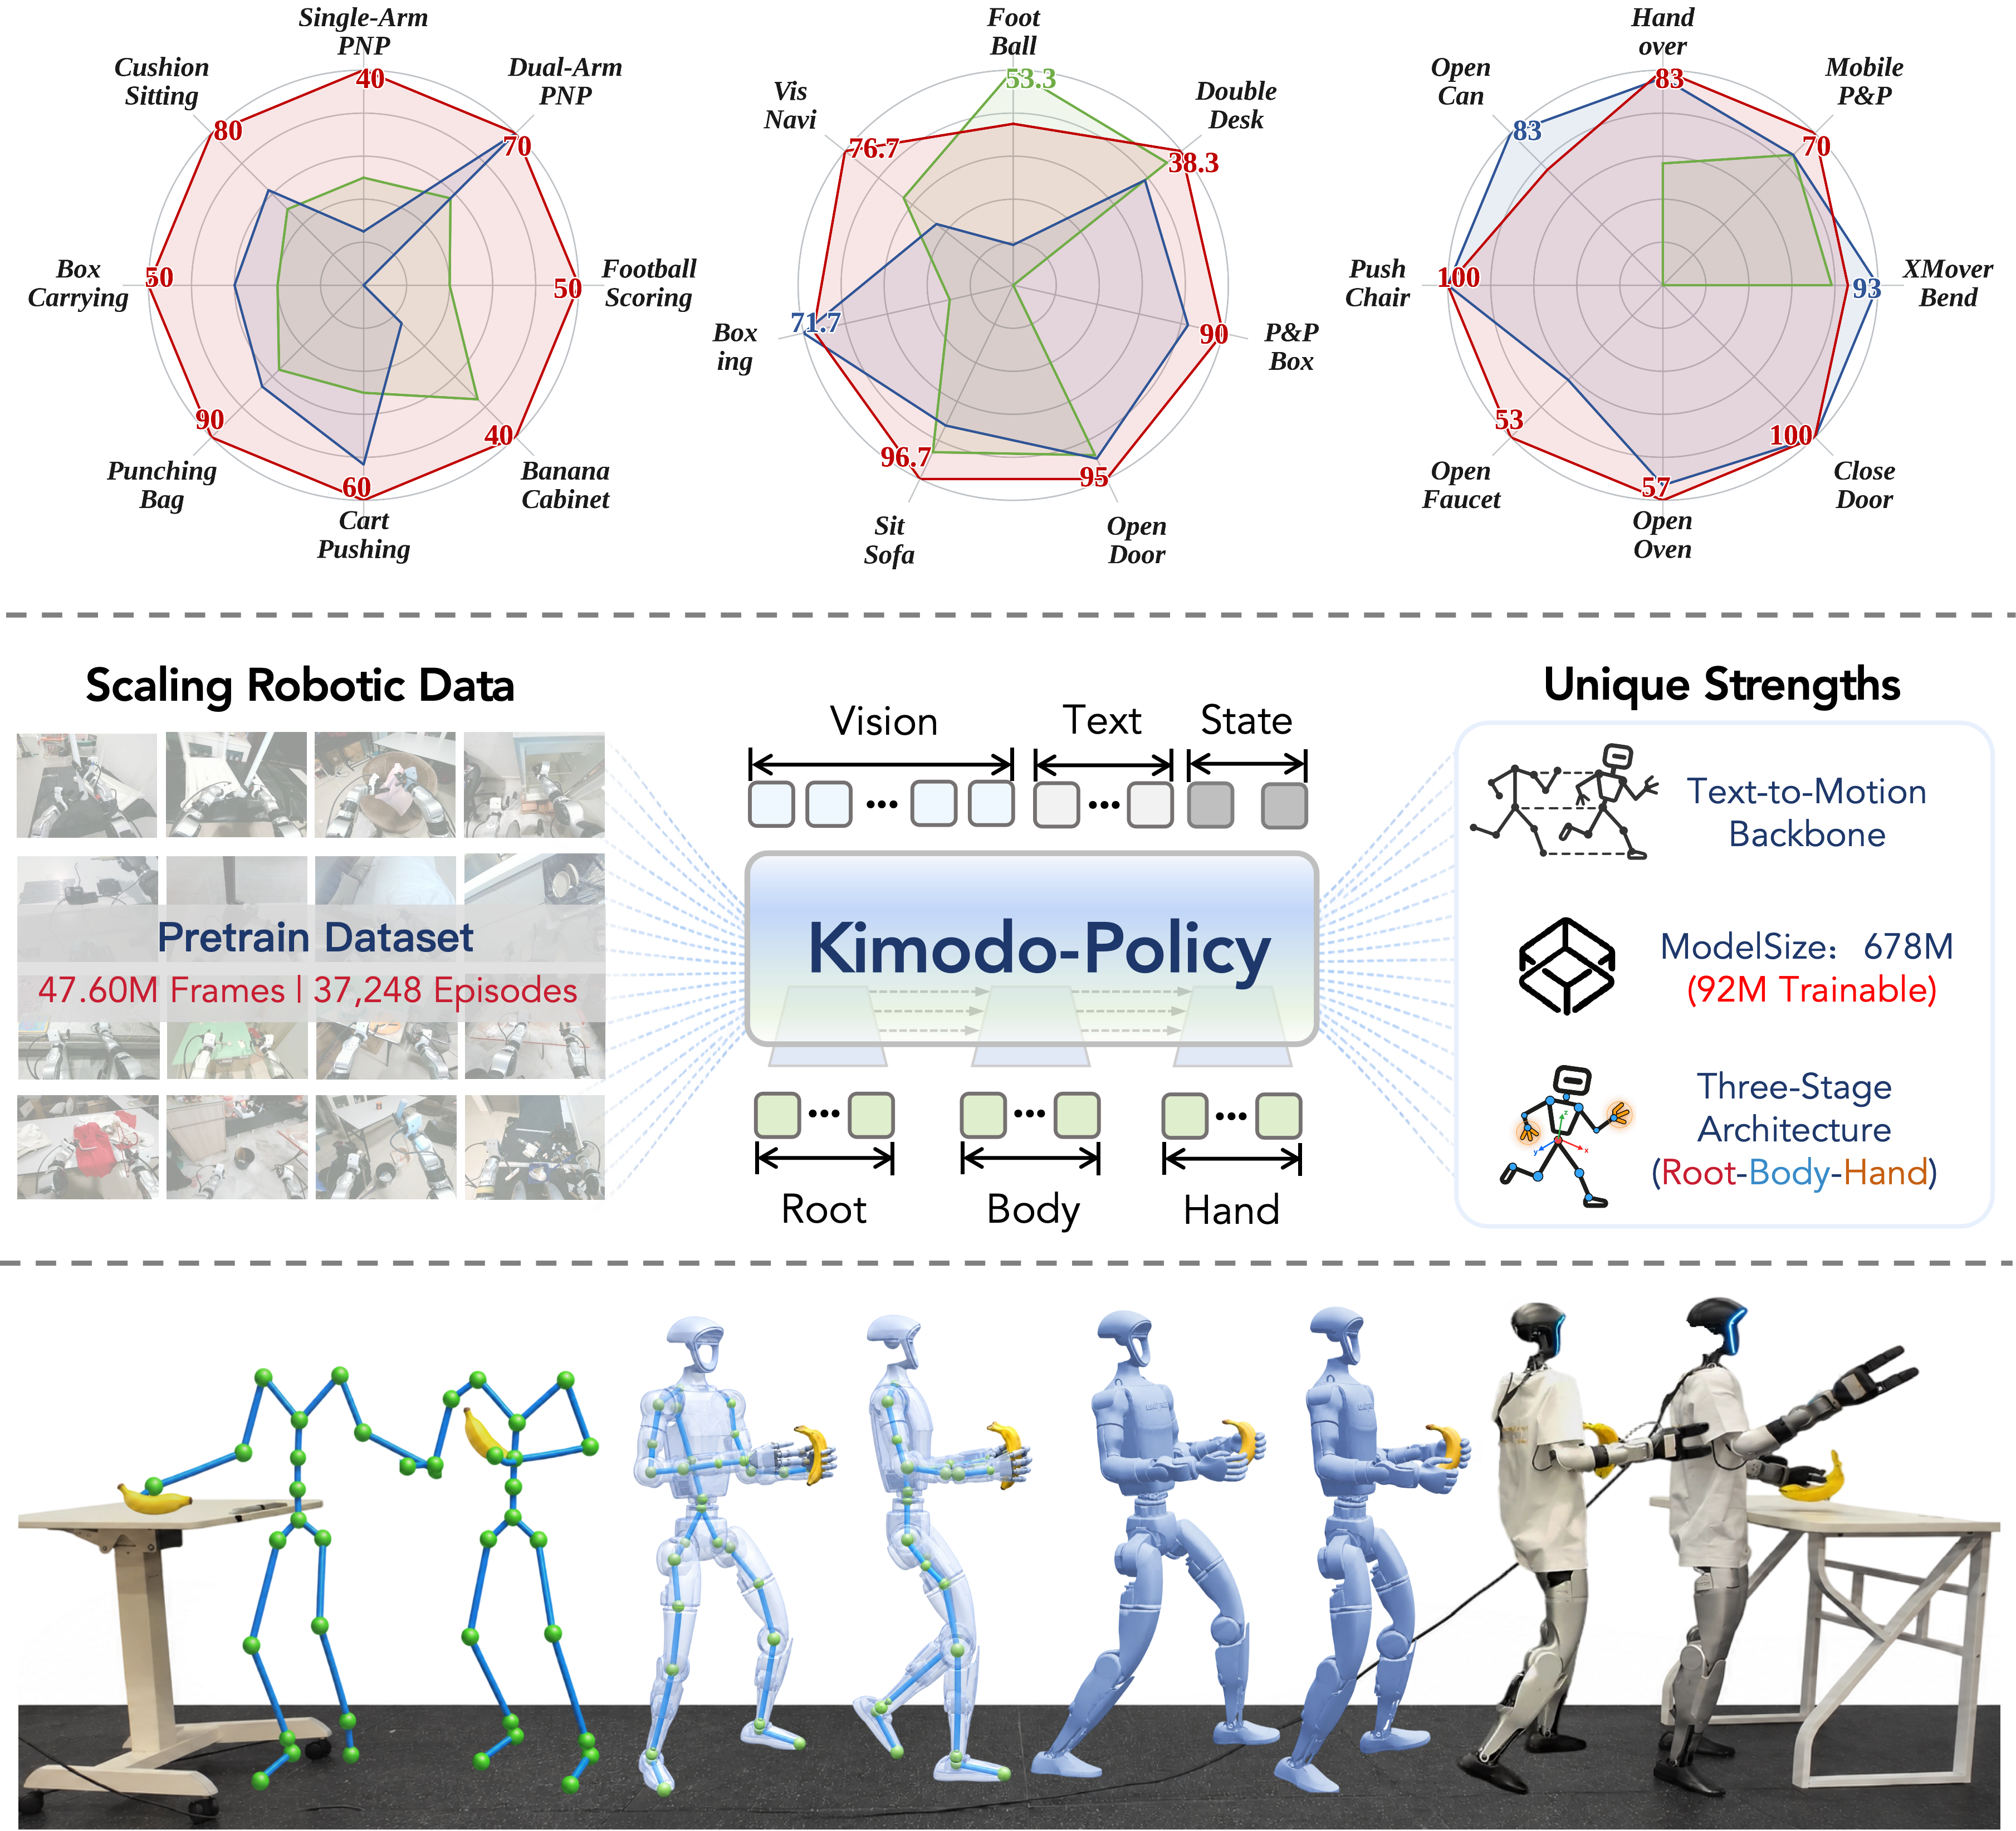
\includegraphics[width=\textwidth]{image/teaser.png}
  \caption{\textbf{Kimodo-Policy as an Instantiation of Kinematic Action Models (KAMs).}
  \textit{Top.} \inlinecolorblock{red!70!black}{red!70!black} Kimodo-Policy, \inlinecolorblock{blue!60!black}{blue!60!black} best baseline, and \inlinecolorblock{green!45!black!65!white}{green!45!black!65!white} second-best baseline. Our KAM-based policy achieves higher mean success than the evaluated VLA and WAM baselines on shared tasks.
  \textit{Middle.} Kimodo-Policy instantiates KAMs by inheriting whole-body motion priors from a pretrained motion generator. The compact policy (678M parameters, 92M trainable) combines large-scale loco-manipulation pretraining with a three-stage root--body--hand architecture.
  \textit{Bottom.} Observed motion history conditions future action-chunk generation for closed-loop control, as demonstrated in real-world object transfer.}
  \label{fig:overview}
\end{figure}
\endgroup

\begin{hclAbstract}
\noindent\textbf{Abstract.}\quad
Vision--language--action models and world action models transfer semantic and visual dynamics priors to robot control, yet humanoid loco-manipulation additionally requires tightly coupled coordination of locomotion, posture, and manipulation. We introduce \textbf{Kinematic Action Models (KAMs)}, a paradigm that uses pretrained motion generation models as the primary backbone for embodied action generation. Motion pretraining supplies reusable whole-body coordination and temporal structure, shifting policy learning toward grounding these priors in perceptual observations, task objectives, and robot state. We instantiate this paradigm with \textbf{Kimodo-Policy}, which combines a frozen Kimodo text-to-motion backbone with lightweight ControlNet-based visual adapters. A three-stage root--body--hand architecture couples global movement, body articulation, and hand control, while motion-history conditioning supports temporally consistent action-chunk generation for closed-loop execution. Large-scale loco-manipulation pretraining adapts the policy to diverse robot interactions. With 678M total parameters and 92M trainable, Kimodo-Policy achieves the highest overall success among evaluated policies on multi-task HumanoidArena (72.14\%), competitive performance on SIMPLE, and 60\% mean success across eight real-world tasks, outperforming the evaluated physical-robot baselines. Ablations support the contribution of motion pretraining, and matched-capacity comparisons show that the choice of motion prior affects downstream performance. These results establish Kimodo-Policy as an initial validation of KAMs for humanoid loco-manipulation.
\end{hclAbstract}


\section{Introduction}
\label{sec:introduction}
% 下面方法是 vlm-based 的人形vla的文章
% https://arxiv.org/pdf/2603.12263
% https://arxiv.org/pdf/2607.18016
% https://arxiv.org/pdf/2503.14734
% https://arxiv.org/pdf/2608.16837
% https://arxiv.org/pdf/2510.03022
% https://arxiv.org/pdf/2606.22174
% https://arxiv.org/pdf/2603.05410
% https://arxiv.org/pdf/2603.09170v1

% 下面方法是 vgm-based 的人形vla 的文章
% https://arxiv.org/pdf/2608.06375
% https://arxiv.org/pdf/2606.09215
% https://arxiv.org/pdf/2609.16644v1

% Local spacing keeps the Introduction and contributions together.
\begingroup
\linespread{0.97}\selectfont
\setlength{\parskip}{0.25em plus 0.05em minus 0.03em}
\setlength{\textfloatsep}{10pt plus 2pt minus 2pt}
\suppressfloats[t]
\begin{figure*}[t]
  \centering
  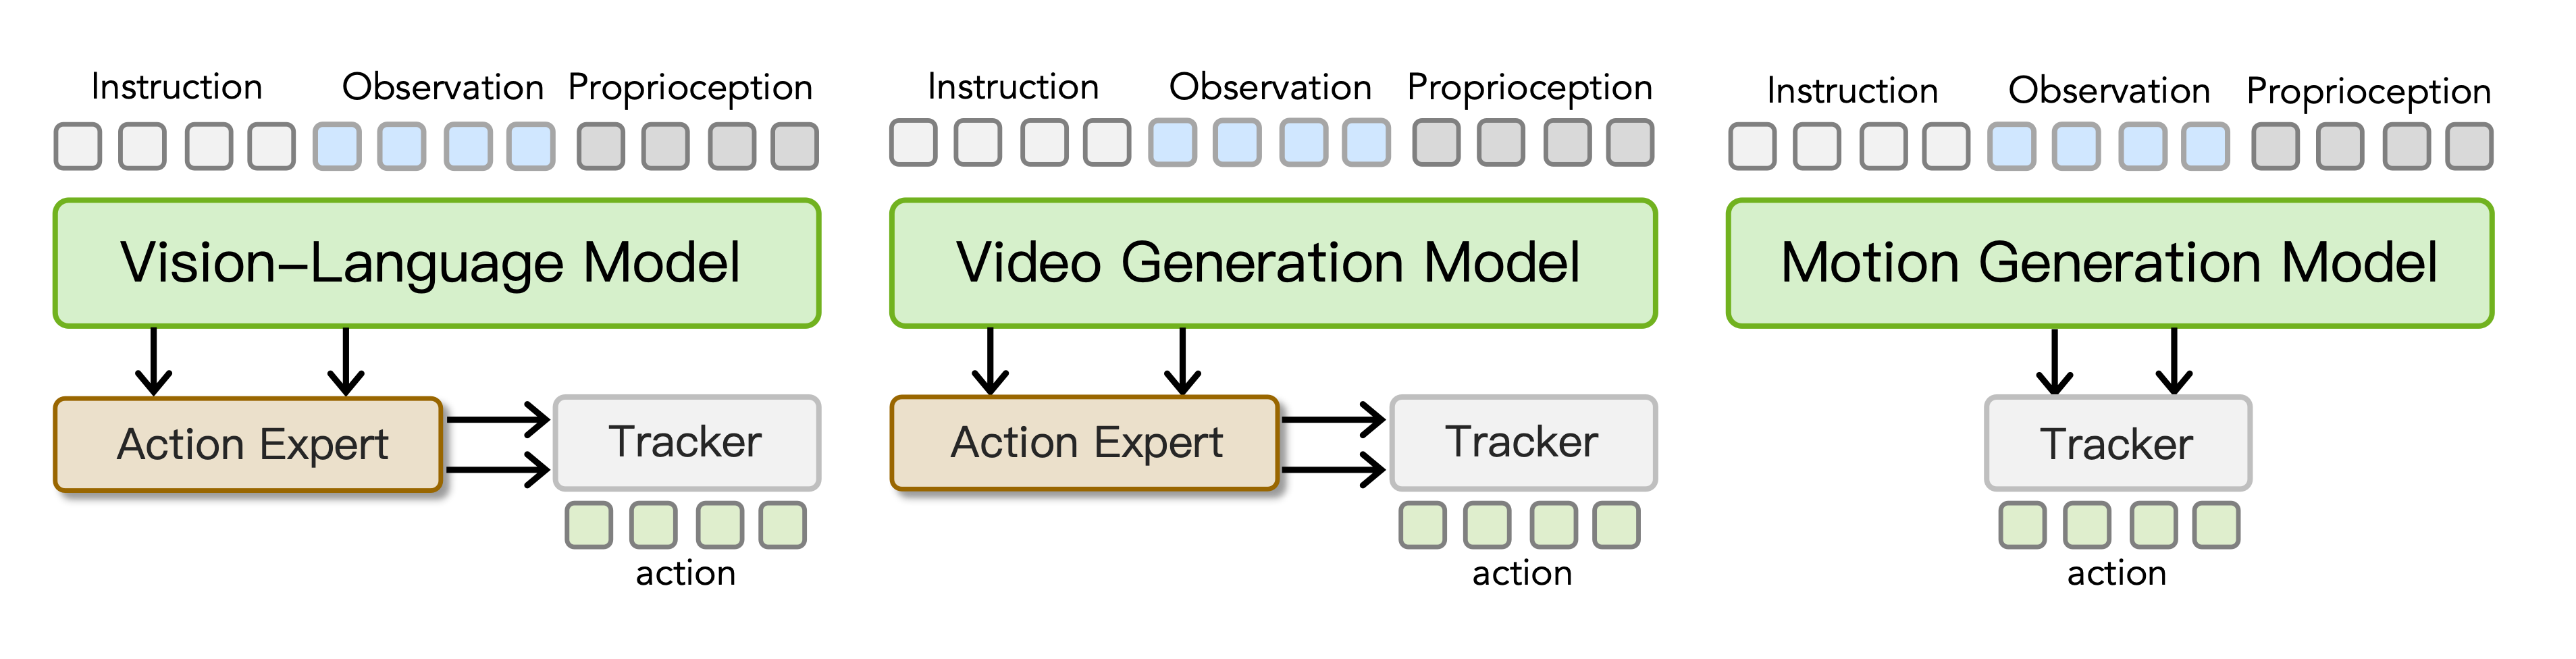
\includegraphics[width=0.98\textwidth]{image/intro.png}
  \caption{\textbf{Pretrained Backbones for Humanoid Action Generation.}
  From left to right: VLA, WAM, and KAM paradigms built around vision--language, video generation, and motion generation models.
  The schematic highlights their primary sources of generative priors: KAMs adapt a pretrained motion generator to produce kinematic action sequences for a downstream tracker, directly transferring learned movement structure into the policy.}
  \label{fig:policy_routes}
\end{figure*}

Humanoid loco-manipulation integrates task understanding, visual perception, and high-dimensional whole-body coordination~\citep{psi0,openhlm}. Beyond the requirements of conventional manipulation, it demands that robots continuously coordinate their root, torso, arms, and legs throughout an interaction~\citep{leverb}. For example, reaching for an object while moving requires a robot to simultaneously adjust its body position, maintain dynamic balance, and coordinate joint movements according to the object's location and contact state. Whole-body motion is therefore an integral part of accomplishing the task, rather than merely an execution stage that follows task-level decision-making. Even with accurate task understanding and perception, a robot cannot complete the task without generating temporally and spatially coordinated, executable whole-body motion. The central challenge of loco-manipulation thus extends beyond determining what the robot should do to generating the high-dimensional, continuous, and coupled whole-body motion required for task execution.

Recent advances in vision--language--action models (VLAs) and world action models (WAMs) offer two representative approaches to robot action generation. VLAs typically extend the semantic understanding and visual representations acquired by pretrained vision--language models to robot action prediction~\citep{rt2,openvla,pi0,grootn1}. WAMs draw on the visual dynamics learned by pretrained video generation models to connect future-state prediction with action generation~\citep{dreamzero,motionwam,wholebodywam_wbc}. These approaches provide important foundations for task understanding, environmental perception, and interaction planning. However, pretrained knowledge of visual semantics and dynamics does not necessarily capture the structural regularities of high-dimensional robot motion. Although these models can acquire whole-body motion capabilities through action supervision and downstream policy learning~\citep{wholebodyvla}, translating visual or semantic representations into coordinated whole-body motion still requires action representations and dependencies that reflect the structure of the robot's motion space. This motivates a complementary question: beyond semantic understanding and visual dynamics, can the structure of whole-body motion itself serve as a distinct target for generative pretraining?

Motivated by this observation, \textit{we introduce Kinematic Action Models (KAMs), a paradigm that uses a pretrained motion generation model as the primary backbone for action generation} (Fig.~\ref{fig:policy_routes}). The central premise of KAMs is that, for humanoid robots whose behavior is expressed through high-dimensional whole-body motion, motion should be a direct target of foundation-model pretraining, in addition to being the final output of a policy. Whereas visual and language pretraining primarily captures visual semantics or the evolution of visual states, motion generation pretraining directly models the temporal evolution of body configurations, learning patterns of joint motion, root motion, and coordination across body parts~\citep{mdm,kimodo}. This allows the model to acquire structural priors in a motion space closely aligned with the target action-generation problem, reducing its reliance on downstream task learning to acquire these basic motion \mbox{regularities}. KAMs then use the pretrained motion generator as the policy's generative backbone, conditioning it on task information, visual observations, and robot states to adapt its existing whole-body motion capabilities to specific environments and objectives. Motion generation thereby becomes a foundation for policy pretraining, rather than solely an output stage following task understanding.

Transferring pretrained motion generation capabilities to robot control nevertheless requires addressing the gap between motion synthesis and closed-loop interaction. Conventional motion generation models typically produce coherent motion sequences from text or kinematic constraints~\citep{mdm,omnicontrol,kimodo}, whereas loco-manipulation requires robots to continually revise their subsequent motion based on current observations and their own states. The challenge is therefore both to acquire priors that capture whole-body coordination and to preserve these priors while making action generation responsive to task requirements and environmental changes. Within this framework, the pretrained motion generator provides reusable whole-body motion structure, perceptual conditioning grounds motion predictions in the current scene and task, and motion history together with continually updated action predictions allows the generation process to incorporate execution feedback. By combining motion structure with task conditioning and closed-loop feedback, KAMs provide a path from general-purpose motion generation to embodied interaction and control.

To investigate this paradigm, we present \textbf{Kimodo-Policy}, an initial instantiation of KAMs for humanoid loco-manipulation (Fig.~\ref{fig:overview}). We combine Kimodo's pretrained text-to-motion backbone~\citep{kimodo} with a lightweight ControlNet-based visual adapter~\citep{zhang2023adding} to directly examine whether strong motion priors can support visually conditioned action generation. The motion backbone remains frozen, while the adapter injects egocentric visual features to guide its predictions. A three-stage root--body--hand architecture first generates a root trajectory, then produces body joint motion conditioned on that trajectory, and finally predicts hand control signals from body features and visual context. Large-scale loco-manipulation pretraining adapts this architecture to robot interaction, while motion-history conditioning and repeated action-chunk prediction support closed-loop execution through a whole-body tracking controller~\citep{sonic}. The resulting policy contains 678 million parameters, of which 92 million are trainable. Across simulation benchmarks and real-robot tasks, Kimodo-Policy achieves the highest overall success rate among the compared policies on multitask HumanoidArena~\citep{humanoidarena}, remains competitive on SIMPLE~\citep{simple}, and outperforms the evaluated baselines on real-world loco-manipulation tasks. Ablation studies support the contribution of the pretrained motion backbone, while comparisons across motion priors show that the choice of pretrained motion model affects downstream performance. These results provide initial evidence that motion generation can serve as a practical foundation for humanoid action models. Our main contributions are threefold:

\begin{samepage}
\begin{itemize}[leftmargin=*,topsep=0pt,itemsep=0.15em,parsep=0pt,partopsep=0pt]
  \item We introduce Kinematic Action Models (KAMs), a paradigm built on pretrained motion generators. By making whole-body motion a direct pretraining target, KAMs transfer temporal and cross-body coordination priors to downstream control, establishing a complementary foundation for humanoid policy learning.
  \item We develop Kimodo-Policy, an initial KAM instantiation with a frozen motion backbone and lightweight visual conditioning. Its root--body--hand hierarchy and motion-history conditioning support closed-loop loco-manipulation in a compact policy with 678M parameters, of which only 92M are trainable.
  \item We achieve the highest overall success among the compared methods on multitask HumanoidArena (72.14\%), competitive SIMPLE performance, and 60\% mean success across eight real-world tasks, outperforming the evaluated real-world baselines. Ablations substantiate the contribution of pretrained motion priors to humanoid control.
\end{itemize}
\end{samepage}
\endgroup


\section{Related Work}
\label{sec:related_work}


% 

\subsection{Humanoid Vision-Language-Action Models}
Humanoid vision--language--action (VLA) models commonly build on pretrained vision--language models (VLMs) or video generation models (VGMs). VLM-based approaches transfer visual-semantic knowledge to action generation~\cite{grootn1,psi0,humanoidexo,openhlm}. For example, GR00T N1~\cite{grootn1} couples a vision--language module with a diffusion action model, while $\Psi_0$~\cite{psi0} transfers representations learned from human egocentric demonstrations to a humanoid action expert. VGM-based approaches exploit visual dynamics priors for action prediction~\cite{motionwam,wholebodywam_wbc}. MotionWAM~\cite{motionwam} conditions whole-body motion generation on intermediate video-model features, while WholeBodyWAM~\cite{wholebodywam_wbc} grounds pretrained world--action priors in whole-body controller interfaces. Across these backbone choices, action organization remains central to whole-body coordination. Unified predictors~\cite{openhlm,motionwam} share a generator across motion components, whereas hybrid interfaces~\cite{humanoidexo,wholebodyvla} combine upper-body targets with locomotion commands. HAF~\cite{haf} further introduces staged generation, using a shared action expert to progressively expand the active action set and refine earlier predictions. Kimodo-Policy instead transfers a pretrained T2M backbone and factorizes generation into dedicated root, body, and hand stages. This design differs in both its pretraining foundation and generative organization: the motion backbone supplies inter-joint coordination and temporal priors, reducing the need to acquire motion regularities from humanoid demonstrations, while specialized generators accommodate distinct control requirements. Explicit cross-stage conditioning connects these generators to support coordinated, visually grounded whole-body behavior.

% 

\subsection{Text-to-Motion (T2M)}
Text-to-motion (T2M) generation has progressed from variational language--motion modeling, exemplified by TEMOS~\cite{temos}, to diffusion- and discrete-token-based formulations. MDM~\cite{mdm} and MLD~\cite{mld} model motion distributions in pose and latent spaces, respectively, whereas T2M-GPT~\cite{t2mgpt} and MoMask~\cite{momask} generate quantized motion tokens through autoregressive prediction and masked modeling. OmniControl~\cite{omnicontrol} extends this line of work with flexible spatial constraints, while Kimodo~\cite{kimodo} scales controllable motion generation through large-scale training and a root--body diffusion hierarchy for human and humanoid skeletons. Related efforts incorporate motion learning into foundation-model adaptation for humanoid control: Humanoid-VLA~\cite{humanoidvla} and ZeroWBC~\cite{zerowbc} learn autoregressive motion priors within pretrained language and vision--language models, respectively, followed by visual integration or task-specific adaptation; MotionWAM~\cite{motionwam} adapts a pretrained video world model through staged video--motion training, whereas WholeBodyWAM~\cite{wholebodywam_motionpriors} pretrains a dedicated motion expert and integrates it with video and action experts. These methods share the goal of transferring motion knowledge to embodied control. Kimodo-Policy instead directly repurposes an existing diffusion-based T2M generator, pretrained on large-scale motion data in the robot's kinematic representation, as the policy's motion-generation backbone.
Our three-stage root--body--hand framework conditions generation on visual observations and motion history for closed-loop loco-manipulation, transferring learned inter-joint coordination and temporal structure to scene-dependent action generation and reducing the need to relearn these regularities from robot demonstrations while accommodating distinct control requirements across motion components.

\section{Preliminaries}
\label{sec:preliminaries}

This section reviews the two foundations of Kimodo-Policy. We first summarize Kimodo's hierarchical text-to-motion formulation and kinematic representation (Sec.~\ref{sec:prelim_kimodo}), and then introduce ControlNet and its parameter-efficient mechanism for injecting additional conditions into a frozen diffusion backbone (Sec.~\ref{sec:prelim_controlnet}).

\subsection{Kimodo}
\label{sec:prelim_kimodo}
\textbf{Architecture Overview.} Kimodo~\cite{kimodo} is a framework for controllable kinematic motion generation based on diffusion, with pretrained models for both the SOMA~\cite{saito2026somaunifyingparametrichuman} human skeleton and the Unitree G1 humanoid robot. Starting from Gaussian noise, it generates motion sequences conditioned on text prompts and optional kinematic constraints using a two-stage Transformer denoiser operating on pose tokens. At each diffusion step $t$, its input--output mapping is summarized as
\begin{equation}
  \widehat{\mathbf{X}}_0 = \mathcal{D}_{\theta}(\mathbf{X}_t,c,t)
  = [\widehat{\mathbf{R}}_0,\widehat{\mathbf{B}}_0].
  \label{eq:kimodo_two_stage}
\end{equation}
Here, $\mathbf{X}_t$ is the noisy motion, $c$ collects the text and motion conditions, and $\widehat{\mathbf{R}}_0$ and $\widehat{\mathbf{B}}_0$ are the predicted clean root and body motions. The denoiser first predicts the global root motion, then uses its local representation to condition body prediction. Text embeddings provide semantic guidance, while masked motion constraints support control through keyframes, joint positions and orientations, and root waypoints or paths. In this work, we primarily use the Kimodo-G1 motion generation model as our pretrained backbone, which is trained on human motion-capture data retargeted to the G1 skeleton using the SOMA retargeter to enable direct generation of kinematic robot motions.

\textbf{Motion Representation.} Kimodo~\cite{kimodo} encodes a motion sequence as $\mathbf{X}=[\mathbf{x}_1,\ldots,\mathbf{x}_N]$ for $N$ frames, with the root at the first frame centered horizontally at the origin. For a skeleton with $J$ joints, each frame contains six groups of kinematic features:
\begin{equation}
  \mathbf{x}_n = [\mathbf{r}^{p}_n,\mathbf{r}^{a}_n,\mathbf{j}^{p}_n,\mathbf{j}^{v}_n,\mathbf{j}^{a}_n,\mathbf{f}_n]
  \in \mathbb{R}^{12J+9}.
  \label{eq:kimodo_motion_representation}
\end{equation}
Here, $\mathbf{r}^{p}_n\in\mathbb{R}^{3}$ is the global root position obtained by smoothing the horizontal $(x,z)$ coordinates of the pelvis while preserving its vertical height, and $\mathbf{r}^{a}_n=[\cos\psi_n,\sin\psi_n]\in\mathbb{R}^{2}$ encodes the global heading angle $\psi_n$. Joint positions $\mathbf{j}^{p}_n\in\mathbb{R}^{3J}$ use horizontal offsets from the smoothed root and absolute vertical coordinates, with axes aligned to the world frame. Joint velocities $\mathbf{j}^{v}_n\in\mathbb{R}^{3J}$ are computed from global joint positions, and joint rotations $\mathbf{j}^{a}_n\in\mathbb{R}^{6J}$ encode each joint's global orientation using a continuous 6D representation. The binary vector $\mathbf{f}_n\in\{0,1\}^{4}$ records contact states for the left heel, left toe, right heel, and right toe. These features form a root component $\mathbf{r}^{\mathrm{glob}}_n=[\mathbf{r}^{p}_n,\mathbf{r}^{a}_n]$ and a body component $\mathbf{b}_n=[\mathbf{j}^{p}_n,\mathbf{j}^{v}_n,\mathbf{j}^{a}_n,\mathbf{f}_n]$, providing an explicit decomposition for root and body motion prediction while supporting spatial constraints on root trajectories, joint positions, and joint orientations.

\subsection{ControlNet}
\label{sec:prelim_controlnet}

\textbf{Architecture Overview.} ControlNet~\cite{zhang2023adding} adapts a pretrained diffusion model to new spatial or semantic conditions while preserving the capabilities acquired by its original backbone. Its central design freezes the pretrained denoiser and adds a trainable control branch with a structurally aligned sequence of layers. The control branch processes the additional condition and produces intermediate features that are injected into the corresponding layers of the frozen branch through zero-initialized projections. For a frozen layer $F_{\ell}$, a trainable control layer $G_{\phi,\ell}$, and condition representation $\mathbf{c}$, the interaction can be written as
\begin{equation}
  \mathbf{h}^{\mathrm{ctrl}}_{\ell+1}
  =G_{\phi,\ell}(\mathbf{h}^{\mathrm{ctrl}}_{\ell},\mathbf{c}),
  \qquad
  \mathbf{h}^{\mathrm{lock}}_{\ell+1}
  =F_{\ell}(\mathbf{h}^{\mathrm{lock}}_{\ell})
  +\mathcal{Z}_{\ell}\!\left(\mathbf{h}^{\mathrm{ctrl}}_{\ell+1}\right),
  \label{eq:controlnet_prelim}
\end{equation}
where $\mathcal{Z}_{\ell}$ is a learnable $1\!\times\!1$ projection initialized to zero. At initialization, the residual path therefore contributes no signal and the adapted model exactly follows the pretrained denoiser. During optimization, gradients update only the control branch and zero projections, allowing the model to learn condition-specific behavior while retaining the original generative prior. This structure is particularly useful when the target dataset is limited or when preserving the motion regularities of a pretrained generator is important. In Kimodo-Policy, we adopt this principle for a transformer-based motion denoiser rather than a convolutional image U-Net~\cite{ronneberger2015unetconvolutionalnetworksbiomedical}. The frozen Kimodo root and body denoisers provide the motion prior, while trainable ControlNet branches receive visual features and inject residual hints at selected denoising layers. The specific visual encoder, dual-path fusion mechanism, and root/body injection strategy are described in Sec.~\ref{sec:method_architecture}.


\section{Method: Kimodo-Policy}
\label{sec:method}
Kimodo-Policy instantiates the KAM paradigm with a pretrained motion backbone and a lightweight visual conditioning mechanism. We use Kimodo~\citep{kimodo} to supply structured root and body motion priors, and ControlNet-based adapters~\citep{zhang2023adding} to ground their generation in egocentric observations. This design provides an initial test of transferring motion generation to closed-loop humanoid loco-manipulation. Appendix~\ref{sec:preliminaries} describes the two components in detail.

\subsection{Model Architecture}
\label{sec:method_architecture}

\textbf{Problem Formulation.} We formulate language-conditioned humanoid loco-manipulation as a closed-loop prediction problem in which the policy generates short, structured action chunks that combine root motion, articulated body motion, and hand controls. At environment step $k$, the policy receives a natural-language instruction $\ell$, the current egocentric RGB image $I_k$, an available motion history $\mathcal{H}_k=[\mathbf{x}_{k-L+1},\ldots,\mathbf{x}_k]$ encoded in the Kimodo representation, and the current bilateral hand state $\mathbf{s}^{h}_k$. It predicts a future chunk of $K$ frames, with each action $\mathbf{a}_i=[\mathbf{r}_i,\mathbf{b}_i,\mathbf{h}_i]$ comprising root motion, articulated body motion, and left/right hand-control signals:
\begin{equation}
  \mathbf{A}_{k+1:k+K}\sim\pi_{\theta}(\,\cdot\mid I_k,\ell,\mathcal{H}_k,\mathbf{s}^{h}_k).
  \label{eq:policy_formulation}
\end{equation}
The root and body components provide kinematic references for a low-level motion tracker~\citep{ze2025twist2scalableportableholistic,guan2026limmtmotiontracking}, while the hand component specifies synchronized closure commands with binary or continuous parameterizations according to the task interface. A prefix of the predicted chunk is executed before replanning from updated observations, allowing visual feedback to guide subsequent motion while the observed history provides temporal context.

\begin{figure}[H]
  \centering
  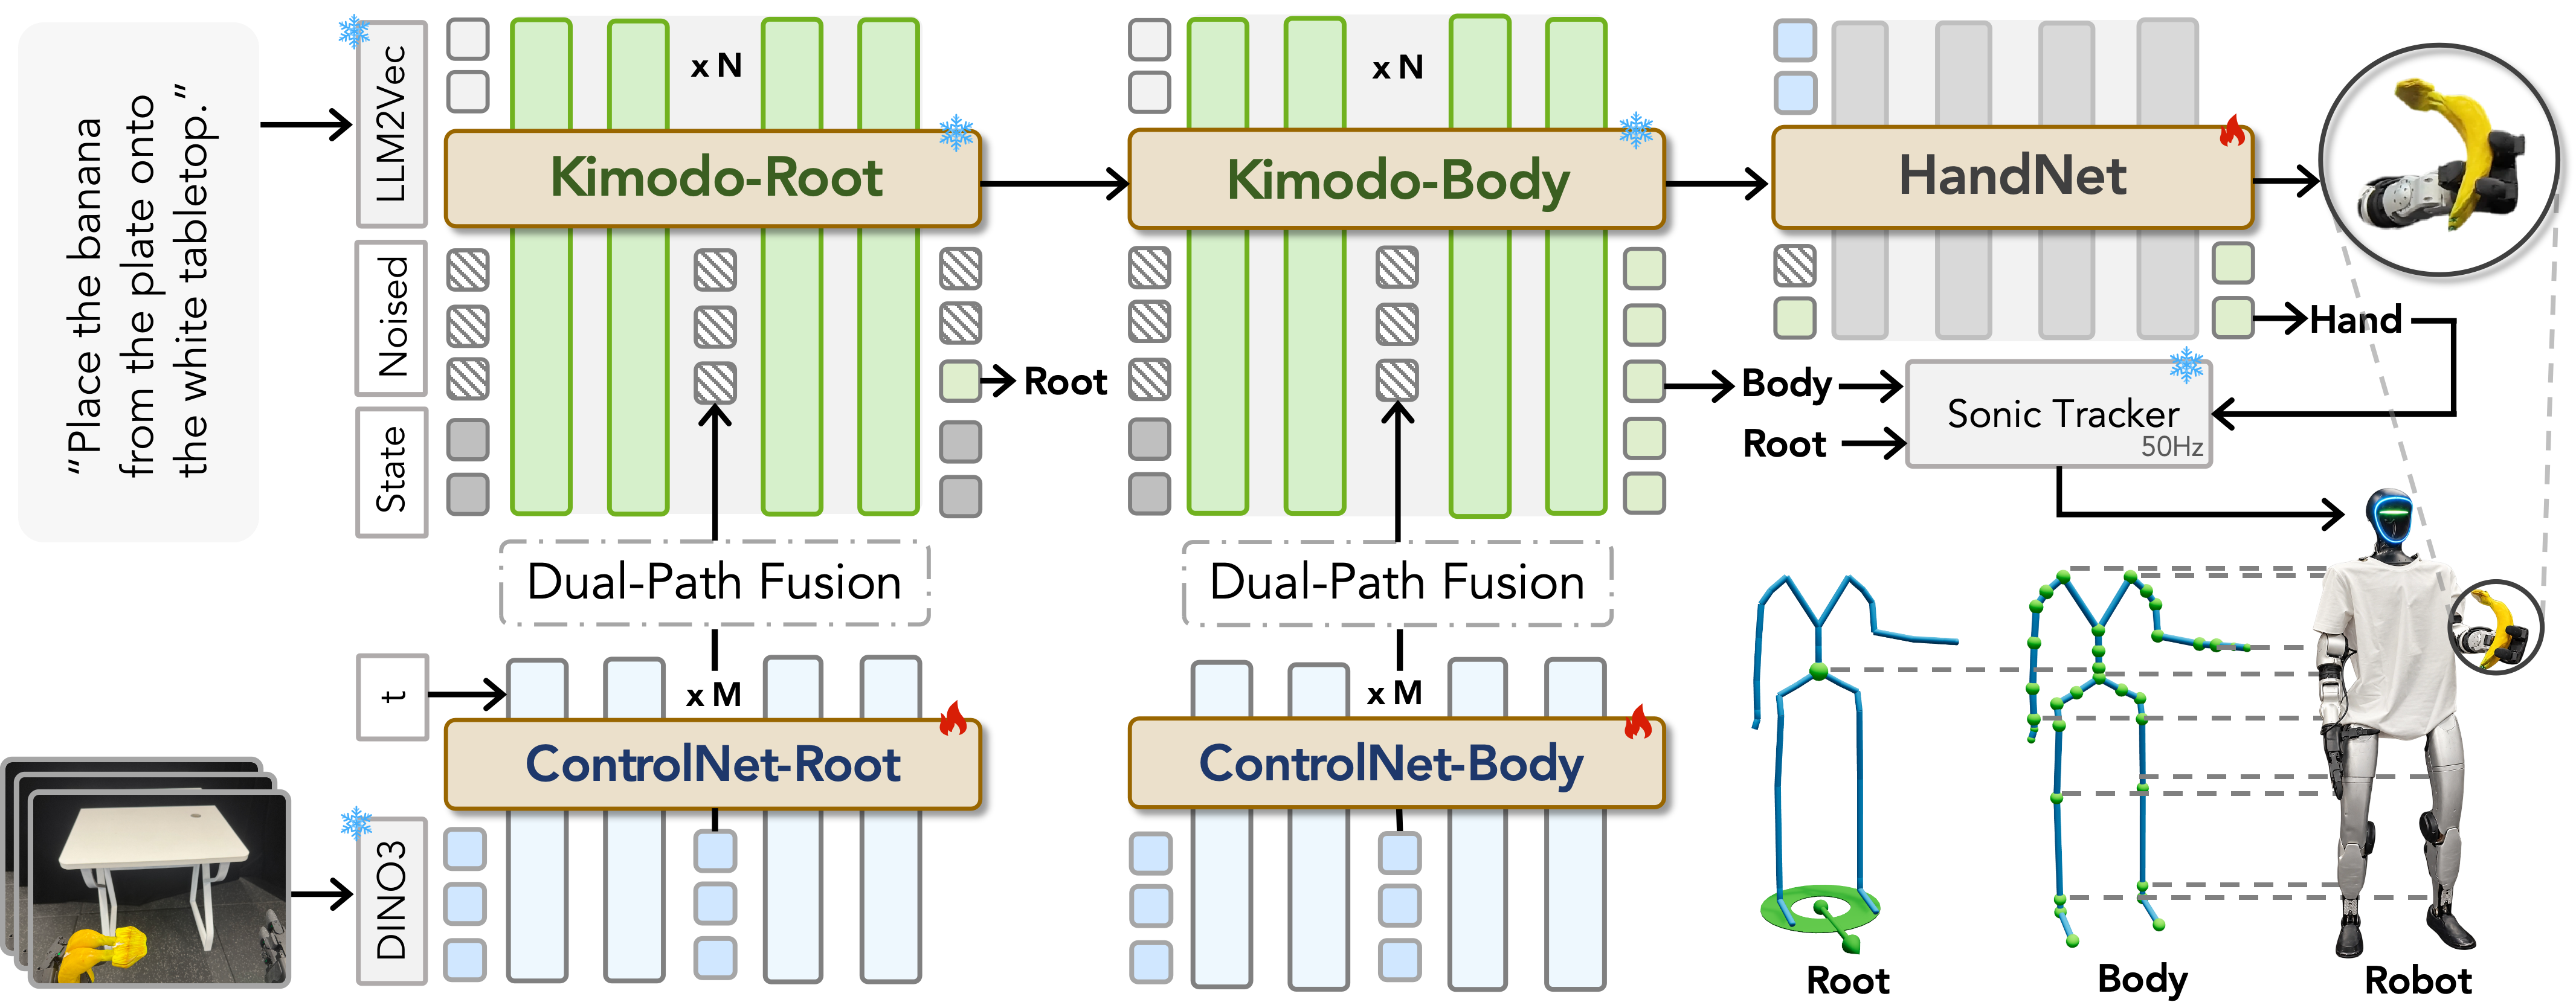
\includegraphics[width=\textwidth]{image/method.png}
  \caption{\textbf{Overview of Kimodo-Policy.} The colored vertical blocks denote \inlinecolorblock{green!55!black}{green!15} ``frozen Kimodo-Root and Kimodo-Body denoisers,'' \inlinecolorblock{blue!55!black}{blue!10} ``trainable ControlNet-Root and ControlNet-Body branches injecting DINOv3~\citep{dinov3} features,'' and \inlinecolorblock{gray!65}{gray!15} ``trainable HandNet denoiser for bilateral hand control.'' Dual-Path Fusion combines motion-query cross-attention with an MLP-based mapping from spatial visual tokens to the future horizon. The predicted root conditions body generation, while future body features condition HandNet; the Motion Projector converts root--body predictions into tracker references. Snowflakes and flames mark frozen and trainable modules, respectively, and dashed boxes indicate Dual-Path Fusion.}
  \label{fig:method_architecture}
\end{figure}

% \textbf{Three-Stage Architecture.} Kimodo-Policy transfers Kimodo's~\citep{kimodo} structured motion prior to visually conditioned humanoid control through a root--body--hand hierarchy. Given the language instruction, egocentric image, and motion history, the root stage predicts global translation and heading; the body stage converts the predicted root to a local representation and generates the articulated whole-body motion conditioned on it. A separate HandNet predicts synchronized bilateral hand controls from the current hand state, visual features, and future body representation. The Kimodo denoiser and DINOv3~\citep{dinov3} encoder remain frozen, while the visual ControlNet branches and HandNet are trainable. As illustrated in Figure~\ref{fig:method_architecture}, this factorization preserves Kimodo's root-to-body kinematic structure, gives hand control a dedicated prediction head, and maps the resulting motion references to a downstream whole-body tracker.

\textbf{Three-Stage Architecture.}
As illustrated in Figure~\ref{fig:method_architecture}, Kimodo-Policy extends Kimodo's~\citep{kimodo} pretrained motion generator into a three-stage root--body--hand architecture.
LLM2Vec~\citep{behnamghader2024llm2veclargelanguagemodels} encodes the instruction, while frozen DINOv3~\citep{dinov3} extracts egocentric visual features.
We retain Kimodo's pretrained root and body denoisers as the motion backbone (Appendix~\ref{sec:prelim_kimodo}). Trainable ControlNet branches inject the visual features into the corresponding frozen denoisers through Dual-Path Fusion (Appendix~\ref{sec:prelim_controlnet}), allowing scene observations to shape future motion within the pretrained kinematic representation.
The inter-stage dependencies are summarized as
\begin{equation}
\mathbf{z}^{r}_k = \mathcal{G}_{r}(\mathbf{c}_k),
\quad
\mathbf{z}^{b}_k = \mathcal{G}_{b}\!\left(\mathbf{c}_k,\operatorname{sg}(\mathbf{z}^{r}_k)\right),
\quad
\widehat{\mathbf{U}}_k = \mathcal{G}_{h}\!\left(\mathbf{s}^{h}_k,\operatorname{sg}(\mathbf{V}_k),\operatorname{sg}(\mathbf{z}^{b}_k)\right),
\label{eq:three_stage_architecture}
\end{equation}
where $\mathbf{c}_k$ collects the instruction embedding, motion history, and visual features $\mathbf{V}_k$;
$\mathbf{z}^{r}_k$ and $\mathbf{z}^{b}_k$ collectively denote each stage's motion predictions and conditioning features;
and $\operatorname{sg}(\cdot)$ denotes stop-gradient.
Sampling noise is omitted for brevity.
The root stage predicts global translation and heading, whose local representation conditions the body stage to generate articulated motion.
The trainable HandNet then combines future body features, visual features, and the current hand state to predict bilateral hand controls $\widehat{\mathbf{U}}_k$.
All root-to-body conditioning is detached, preventing body-stage gradients from reaching either Kimodo-Root or ControlNet-Root.
Likewise, body and visual features supplied to HandNet are detached, preventing hand supervision from updating Kimodo-Body or the ControlNet branches.
These gradient boundaries separate optimization across the three stages while preserving their forward dependencies for coordinated generation.
Finally, root and body predictions are converted into whole-body tracking references and executed alongside the hand commands.

\textbf{Dual-Path Fusion.} To ground the frozen motion prior in the current scene, we encode the egocentric image into spatial tokens with DINOv3~\citep{dinov3} and process them through trainable root and body ControlNet branches. At selected layers of each Kimodo denoiser, we fuse visual context through two complementary paths. In the cross-attention path, future-motion hidden states serve as queries over the image tokens, allowing each predicted time step to retrieve task-relevant visual evidence. In parallel, a token-axis MLP maps the spatial image-token sequence to the future temporal horizon, providing a direct image-to-time correspondence. We sum the two outputs and pass them through a layer-specific zero-initialized projection to form a residual hint for the corresponding Kimodo layer. These hints are added only to future-motion tokens, leaving the constrained history prefix unchanged. The zero initialization preserves the pretrained denoiser's behavior at the start of adaptation, while the two paths jointly support content-selective visual retrieval and temporally aligned conditioning.

\textbf{HandNet.} Hand control has different output semantics from root and body motion: it specifies when each hand should open or close, rather than a kinematic pose trajectory. We therefore model bilateral hand control with a dedicated diffusion head. At each denoising step, HandNet jointly processes the current hand state, noisy future hand controls, future body hidden states, and visual tokens, and predicts two hand-control values for every future frame. Conditioning on the predicted body and current scene aligns interaction commands with the evolving whole-body action, while a separate head avoids placing hand labels in the root--body motion space. The head supports binary open/close states and continuous closure changes. During training, its body and visual conditioning features are detached, so hand supervision updates HandNet without sending gradients into the motion denoiser or ControlNet.

\subsection{Adapting Motion Priors for Closed-Loop Control}
\label{sec:t2m_transfer}

\textbf{Motion Prior Transfer.} Figure~\ref{fig:t2m_transfer} illustrates the role of the pretrained generator in this instantiation of KAM. Given the instruction ``Sit on the sofa,'' Kimodo~\citep{kimodo} produces a coordinated sitting sequence (top row). This sequence provides a prior over the temporal relationship between root motion and body posture. For execution, visual conditioning adapts the motion to the observed scene, while motion history anchors the prediction to the robot's ongoing trajectory. The resulting policy performs the same behavior using egocentric observations and state history (bottom row). The example illustrates how the policy can reuse pretrained coordination and learn to ground it in a particular interaction from robot demonstrations.

\begin{figure}[H]
  \centering
  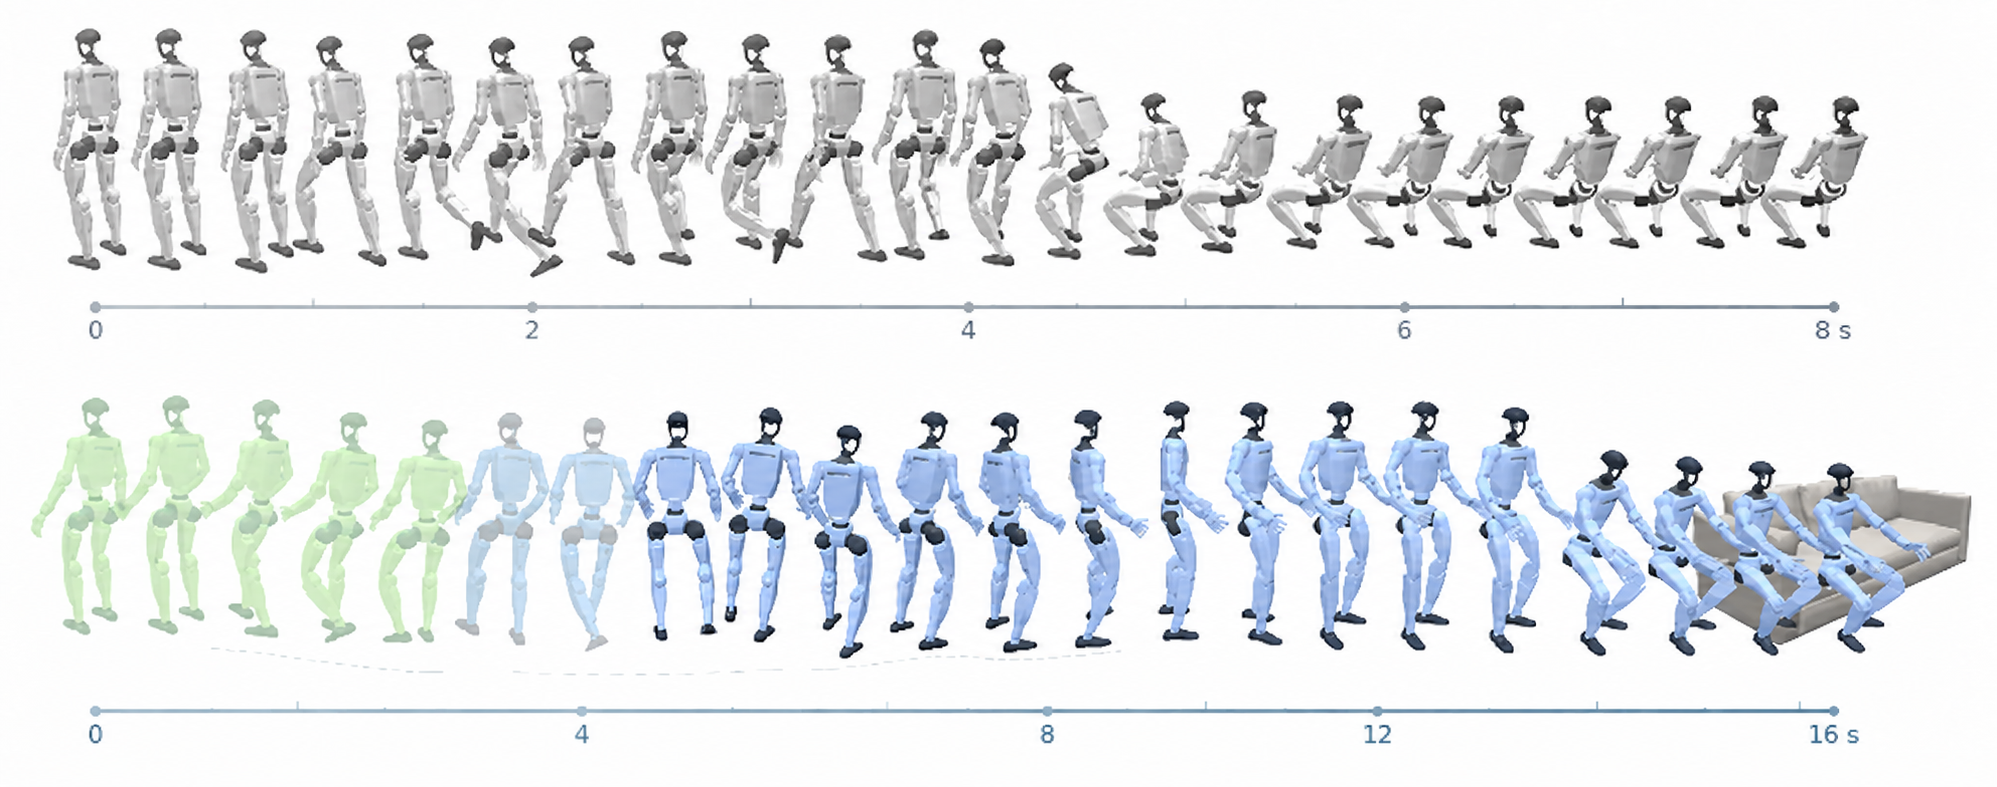
\includegraphics[width=\textwidth]{image/method_22.png}
  \caption{\textbf{Motion-Prior Transfer for Closed-Loop Control.} Top: frozen Kimodo generates a complete ``Sit on the sofa'' sequence from text alone. Bottom: Kimodo-Policy grounds the same prior with visual observations and motion history, repeatedly predicting short action chunks for closed-loop execution. Light-green poses denote observed history; blue poses denote predicted and executed motion.}
  \label{fig:t2m_transfer}
\end{figure}

\textbf{Motion-History Conditioning.} Adapting text-to-motion generation to closed-loop VLA control entails a temporal mismatch: a T2M model is designed to synthesize a coherent motion sequence over an extended horizon, whereas a robot policy must repeatedly predict a finite action chunk, execute only part of it, and revise its prediction in response to new observations. Replaying a sequence generated once cannot account for deviations between predicted and measured motion or changes in the visual scene. We address this mismatch by formulating each policy query as constrained motion completion in Kimodo's kinematic representation. At every replanning step, the observed motion history is placed in the prefix of a history--future window, and a feature-wise mask specifies which kinematic values are available. The observed prefix is restored before each denoising step, while the unconstrained future is generated as the next action chunk. In parallel, trainable ControlNet branches inject features from the current egocentric image into Kimodo's root and body denoisers, grounding the generated motion in the scene while retaining the pretrained root--body structure. The policy executes a prefix of the predicted chunk through the motion tracker; the resulting state history and updated image then condition the next prediction. This formulation turns Kimodo's constraint-conditioned sequence generator into a receding-horizon controller, preserving its structured motion prior while enabling continual visual and state-based correction.

\subsection{Training and Inference}
\label{sec:training_inference}

\textbf{Training Objective.} We train the ControlNet branches and HandNet with supervised denoising on demonstration windows. For each window, we sample a diffusion timestep and perturb the normalized root--body features and hand targets with Gaussian noise. A feature-wise mask imposes the observed history as a constraint, while supervision is applied to valid future frames. The objective is
\begin{equation}
  \mathcal{L}=\lambda_r\mathcal{L}_{r}+\lambda_b\mathcal{L}_{b}
  +\lambda_h\bigl(\mathcal{L}_{h}+\lambda_{\Delta}\mathcal{L}_{\Delta}\bigr),
  \label{eq:policy_training_objective}
\end{equation}
where $\mathcal{L}_{r}$ and $\mathcal{L}_{b}$ are masked mean squared errors between the predicted clean root and body features, respectively, and their normalized targets, evaluated over valid future frames. For binary control, hand states are encoded in $[-1,1]$; for continuous control, HandNet predicts closure residuals relative to the latest valid observed hand state. The hand reconstruction loss $\mathcal{L}_{h}$ is a masked mean squared error on these targets. The transition loss $\mathcal{L}_{\Delta}$ penalizes the $\ell_1$ error between predicted and demonstrated consecutive hand-control changes, including the transition from the observed state to the first future frame. In continuous mode, predicted residuals are converted back to closure values before computing this loss. Motion losses exclude padded frames, while hand losses additionally mask unavailable labels; transition terms are evaluated only when both adjacent labels are valid. For the main MSE configuration, we use $(\lambda_r,\lambda_b,\lambda_h,\lambda_{\Delta})=(4,1,1,0.2)$. We detach the predicted root before body generation and, in the main configuration, detach root ControlNet features passed to the body branch. HandNet also receives detached body and visual features. These detachments regulate gradient flow between trainable branches, while the Kimodo denoisers and DINOv3~\citep{dinov3} encoder remain frozen.

\textbf{Inference.} At each policy query, we encode the language instruction and current egocentric image, and represent the available proprioceptive history in Kimodo's motion space with frame- and feature-wise observation masks. We initialize the future motion and hand sequences from Gaussian noise and iteratively denoise them with DDIM~\citep{song2022denoisingdiffusionimplicitmodels}. At each step, the observed history is restored, visual features are injected into the frozen root and body denoisers through ControlNet, the predicted root conditions body generation, and HandNet predicts hand controls from the current hand state, visual features, and future body features. After the final denoising step, we invert the motion representation and map the resulting root and joint trajectories, together with bilateral hand commands, to tracker-compatible references. The low-level whole-body tracker executes a prefix of the predicted chunk; the policy then incorporates the updated visual observation and proprioceptive state to replan. This receding-horizon loop combines structured motion generation with continual closed-loop correction.


\section{Experimental Setup}
\label{sec:experimental_setup}

This section describes the data, training protocols, and evaluation environments used to assess Kimodo-Policy. We first detail VLA policy pretraining on heterogeneous humanoid demonstrations (Sec.~\ref{sec:setup_pretraining}), and then describe post-training and evaluation on the HumanoidArena and SIMPLE simulators as well as on a physical humanoid robot (Sec.~\ref{sec:setup_posttraining}).

\subsection{Pretraining}
\label{sec:setup_pretraining}
\textbf{Dataset.} We assemble a 419-hour pretraining corpus from three publicly released humanoid datasets (Fig.~\ref{fig:pretraining_datasets}). HIW-500 provides teleoperated Unitree G1 demonstrations collected in real homes. From UniFoLM-WBT, we use the 14 task-specific G1 subsets available when our corpus was assembled: the BrainCo subsets \emph{Collect Plates into Dishwasher}, \emph{Make the Bed}, \emph{Pick Up Medicine}, and \emph{Pickup Pillow}; the Dex1 subset \emph{Put Clothes into Washing Machine}; and the Inspire subsets \emph{Clean the Living Room}, \emph{Collect Clothes (MainCamOnly)}, \emph{Pick Up Drinks}, \emph{Pickup Pillow (MainCamOnly)}, \emph{Put Clothes into Basket}, \emph{Put Clothes into Washing Machine}, \emph{Put Clothes into Washing Machine (MainCamOnly)}, \emph{Put Drinks into Fridge}, and \emph{Put Vegetables into Basket}. Main-camera-only variants are included when available, while UniFoLM-WBT entries released after this snapshot are excluded. Humanoid Everyday~\cite{humanoid_everyday} contributes 10.3K trajectories, over three million frames, and 260 tasks spanning dexterous manipulation, articulated-object interaction, human--robot interaction, and locomotion-integrated behaviors. We form training examples from an egocentric image, a language instruction, a 100-frame motion history, and a 50-frame future action chunk sampled at 30~Hz, converting trajectories to Kimodo's motion representation.

\begin{figure}[H]
  \centering
  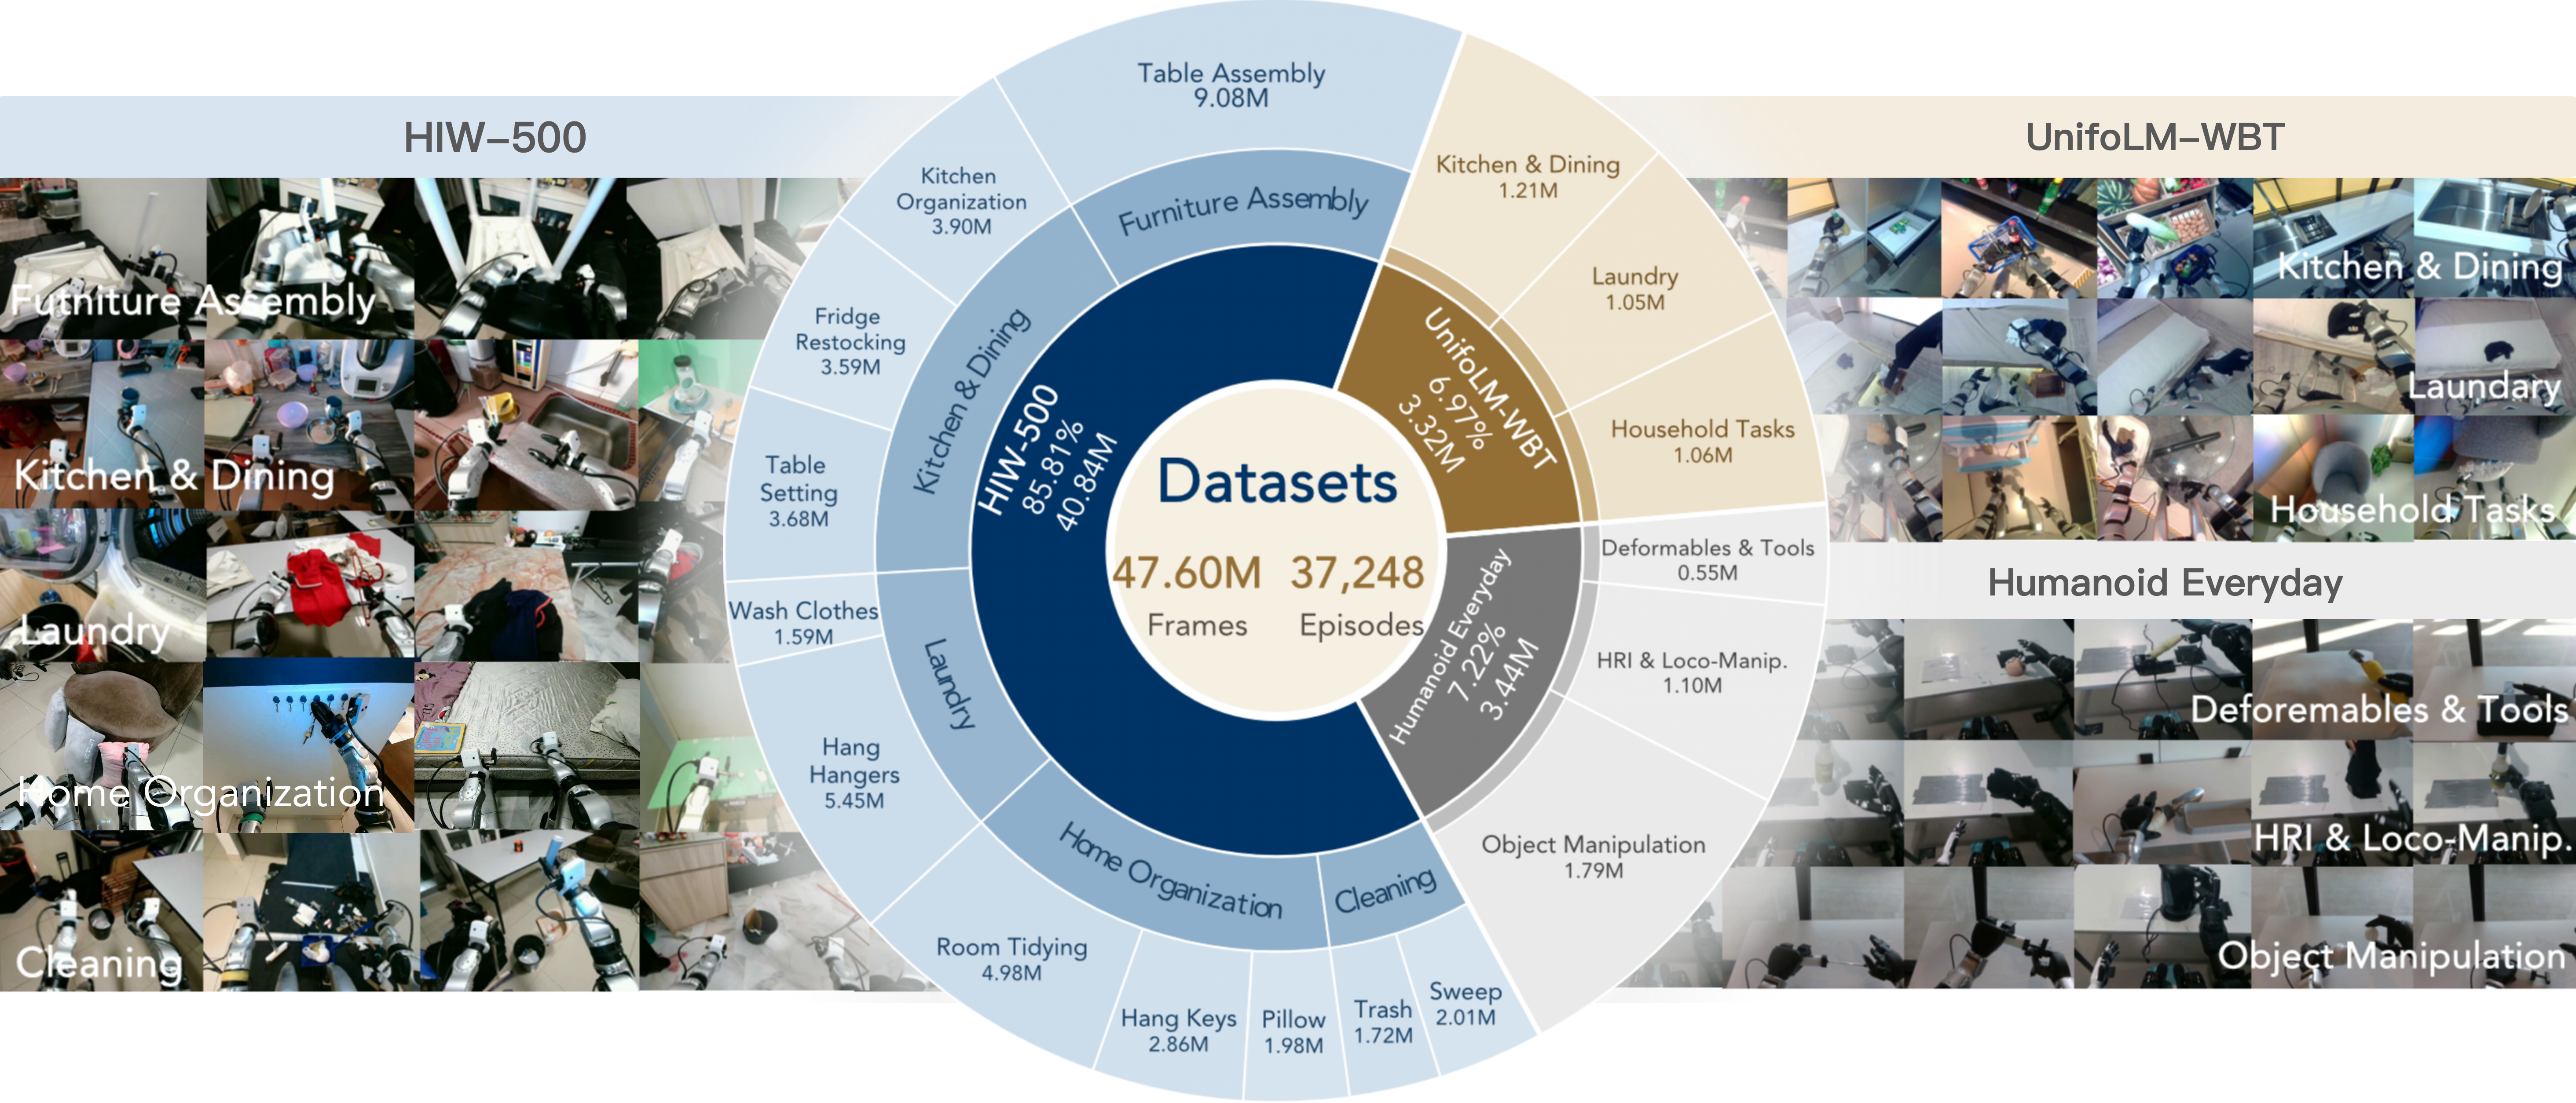
\includegraphics[width=\textwidth]{image/pretrain.png}
  \caption{\textbf{Composition of the VLA Pretraining Corpus.} The corpus combines HIW-500, 14 task subsets from UniFoLM-WBT available when the corpus was assembled, and Humanoid Everyday. UniFoLM-WBT entries released after corpus construction are excluded.}
  \label{fig:pretraining_datasets}
\end{figure}

\textbf{Implementation Details.} We pretrain the policy for 1,000k optimization steps on 16 NVIDIA H200 GPUs, taking approximately 60 hours with bfloat16 mixed precision and a global batch size of 1024. During VLA pretraining, hand supervision is represented as a two-dimensional binary vector indicating the open/closed state of the left and right hands. This shared representation accommodates the different hand morphologies, degrees of freedom, and control conventions in the source datasets, preserving grasp-and-release semantics while providing a consistent target for the hand head. We use AdamW with learning rates of $3\times10^{-5}$ for the ControlNet backbone and $1\times10^{-4}$ for the ControlNet adapters and hand head, together with a weight decay of $0.01$. The learning rate follows a cosine schedule with 1\% warm-up and a minimum of 10\% of its initial value.

\subsection{Post-Training}
\label{sec:setup_posttraining}
\textbf{HumanoidArena Benchmark.} HumanoidArena~\cite{humanoidarena,sonic} provides seven leg-critical tasks: three human--object and four human--scene interaction tasks requiring coordinated locomotion, balance, posture adjustment, and manipulation. Its SONIC data contain 100 successful demonstrations per task (700 total) with synchronized egocentric RGB, proprioceptive states, and whole-body targets. We use all seven tasks for single-task fine-tuning and joint multi-task training, the latter being more challenging because one policy must acquire all tasks simultaneously. We evaluate closed-loop performance with SONIC using success rate (SR) and average fall rate (AFR), capturing both task completion and stability during whole-body task execution.

\textbf{SIMPLE Benchmark.} SIMPLE~\cite{simple} integrates MuJoCo contact dynamics with Isaac Sim rendering for scalable evaluation of humanoid loco-manipulation. The paper describes a benchmark comprising 60 tasks; of these, 18 have been released in the public codebase to date. The paper reports baseline results for six tasks, with two evaluated using AMO and four using the SONIC tracker. From the currently released tasks, we select eight for evaluation: Handover, Mobile P\&P, XMoveBendPick, CloseDoor, OpenOven, OpenFaucet, Push Office Chair, and OpenTrashCan. Together, these tasks cover object handover, mobile pick-and-place, articulated-object interaction, and household-object manipulation, allowing us to assess policy robustness and execution stability in contact-rich whole-body control.

\textbf{Real-World Data Collection and Setup.} We collect real-world demonstrations with a teleoperation system implemented on top of and extended from the NVIDIA Isaac-GR00T data-preparation pipeline~\cite{grootn1}. As shown on the left of Fig.~\ref{fig:real_world_setup}, the operator uses a PICO 4 Ultra headset and hand controllers together with PICO body trackers for whole-body and lower-limb tracking. The humanoid is equipped with an Intel RealSense D435i camera and Dex3-1 dexterous hands. We define eight real-world tasks spanning locomotion, balance, and single- and dual-arm manipulation, and record 25--30 demonstrations per task. The two plots on the right of Fig.~\ref{fig:real_world_setup} show representative joint-position traces from two of these tasks: in Football Scoring (Fig.~\ref{fig:real_world_setup}a), the right-leg trajectory changes sharply around the kick, while in Banana Cabinet (Fig.~\ref{fig:real_world_setup}b), the traces vary across the pick, place, and push phases. In both plots, solid curves show measured joint positions and dashed curves show the corresponding action commands for the left and right sides, illustrating the task-dependent motion captured in the demonstrations. We store the demonstrations in a LeRobot v2.1~\cite{cadene2026lerobotopensourcelibraryendtoend}-compatible format, extended with Kimodo-specific motion and control fields for policy training with a motion prior.

\begin{figure}[H]
  \centering
  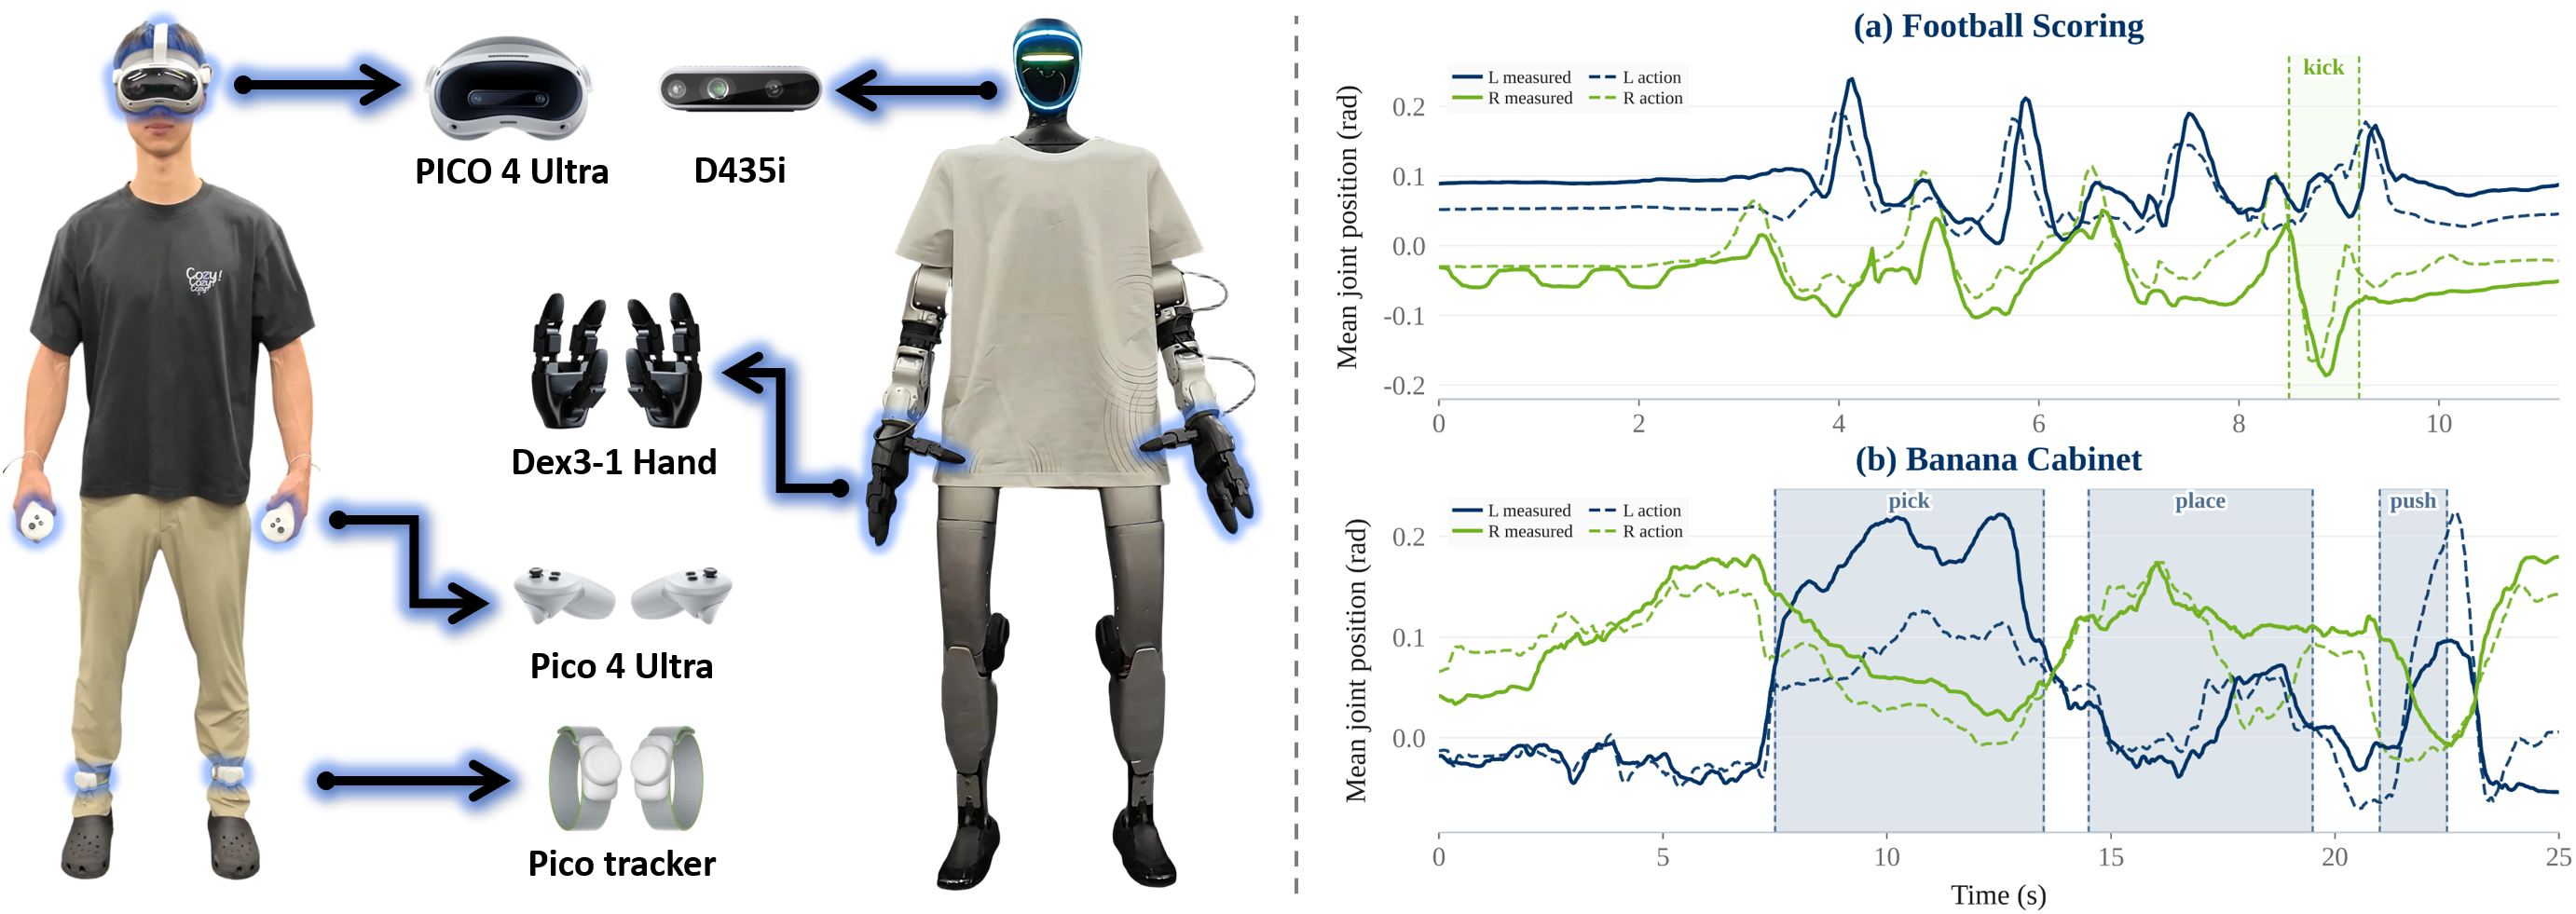
\includegraphics[width=\textwidth]{image/post-train.png}
  \caption{\textbf{Real-World Data Collection and Motion Profiles.} Left: PICO-based whole-body teleoperation of the humanoid. Right: measured (solid) and commanded (dashed) left- and right-side mean joint positions for two of the eight physical-robot tasks: (a) Football Scoring, showing a pronounced right-leg change during the kick, and (b) Banana Cabinet, showing motion across the pick, place, and push phases.}
  \label{fig:real_world_setup}
\end{figure}

\textbf{Implementation Details.} We fine-tune all policies with bfloat16 precision on four GPUs using 30\,Hz motion sequences, a 100-frame history, and a 50-frame prediction horizon. HumanoidArena single-task policies use a global batch size of 64 for 200k steps, while the joint seven-task policy uses a batch size of 128 for 500k steps; SIMPLE uses a batch size of 64 for 200k steps, and real-world policies use a batch size of 32 for 50k steps. Scratch-trained and VLA-pretrained variants share the same fine-tuning setup and differ only in initialization. The four-layer ControlNet detaches the root-control input to body prediction. We train with an MSE objective weighted 4, 1, 1, and 0.2 for root motion, body motion, hand control, and hand transitions, respectively, using AdamW (weight decay 0.01) and a cosine schedule with 1\% warm-up and a 10\% minimum learning-rate ratio. The ControlNet backbone, adapters, and hand head use learning rates of $3\times10^{-5}$, $1\times10^{-4}$, and $1\times10^{-4}$ for HumanoidArena and real-world fine-tuning, and $1\times10^{-5}$, $3\times10^{-5}$, and $3\times10^{-5}$ for SIMPLE. SIMPLE training uses color jitter and continuous hand-control targets; real-world training uses color jitter and random crops, with binary hand commands conditioned on measured hand closure. At inference, all policies run on one NVIDIA RTX 4090 with 10 diffusion denoising steps and predict a 50-frame action horizon at 30\,Hz. We execute 15 predicted frames per policy update on HumanoidArena and the real robot, and either 15 or 50 frames on SIMPLE depending on the evaluation setting. The SONIC tracker runs at 50\,Hz; real-time correction (RTC)~\cite{rtc} is enabled only for real-world deployment and disabled for HumanoidArena and SIMPLE.


\section{Experimental Results}
\label{sec:experiments}

We evaluate motion generation as a foundation for humanoid control through benchmark and real-world experiments (Secs.~\ref{sec:exp_simulation}--\ref{sec:exp_real}), followed by analyses of motion priors, scaling, and adaptation design (Secs.~\ref{sec:exp_t2m}--\ref{sec:exp_ablation}). Unless explicitly ablated, all Kimodo-Policy variants retain the pretrained motion backbone. Kimodo-Policy denotes direct downstream fine-tuning, while Kimodo-Policy$^{*}$ additionally initializes the conditioning modules and hand head through policy pretraining on 419 hours of robot-interaction data.

\subsection{Evaluation on the HumanoidArena Benchmark}
\label{sec:exp_simulation}

HumanoidArena~\citep{humanoidarena} comprises seven language-conditioned tasks spanning human--object interaction (HOI) and human--scene interaction (HSI), with substantial requirements for locomotion, posture adjustment, and manipulation (Fig.~\ref{fig:humanoidarena}). We evaluate both independent task-specific policies and a single policy jointly trained on all seven tasks. Success rate (SR) measures task completion, while average fall rate (AFR) characterizes execution stability within the SONIC-based control stack~\citep{sonic}. Real-time chunking (RTC) is disabled in our simulation evaluations.

\begin{figure}[H]
  \centering
  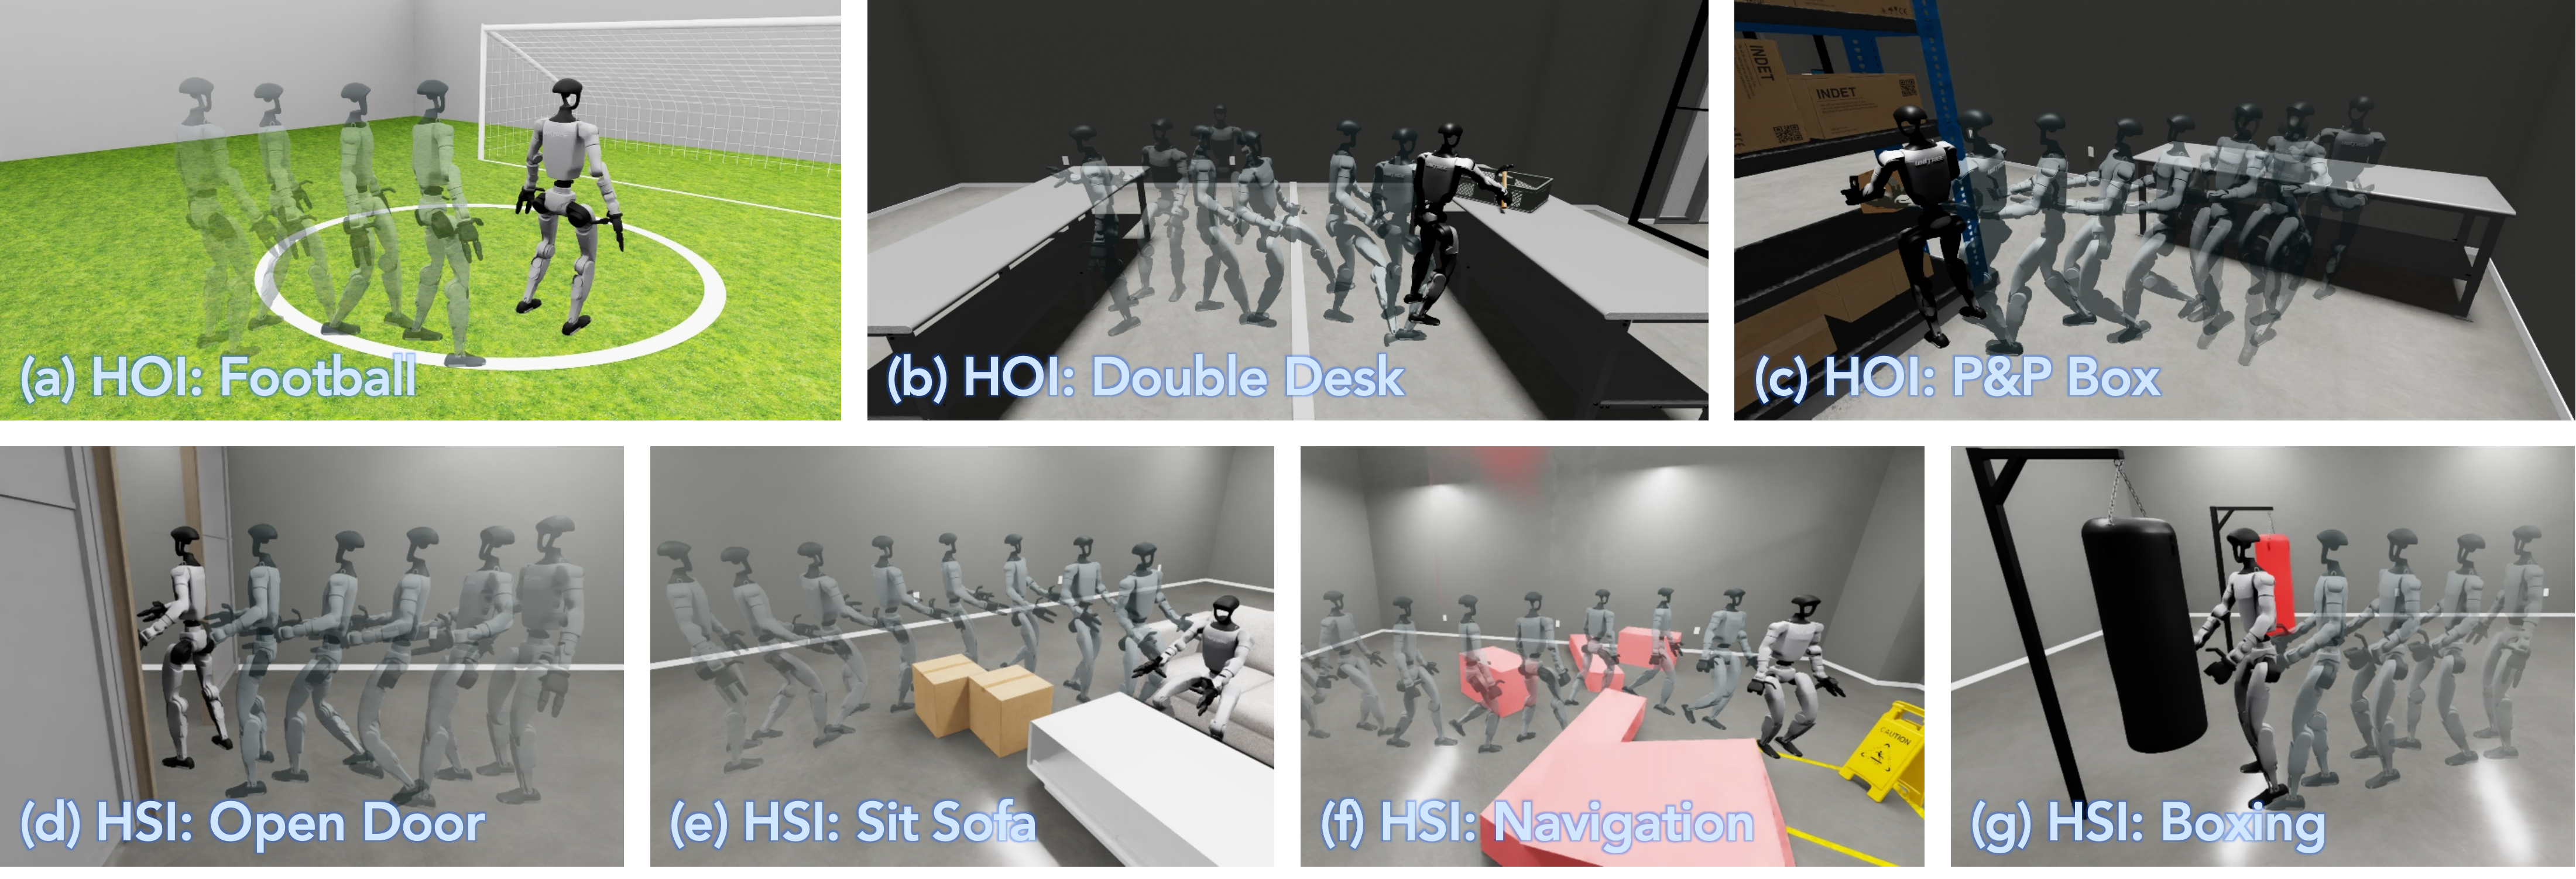
\includegraphics[width=\textwidth]{image/arena.png}
  \caption{\textbf{Visualization of the Seven HumanoidArena Tasks.} The benchmark includes Football, DoubleDesk, P\&Pbox, OpenDoor, SitSofa, Boxing, and VisNavi, covering language-conditioned humanoid behavior across human--object and human--scene interaction with coordinated locomotion, balance, and manipulation.}
  \label{fig:humanoidarena}
\end{figure}

\textbf{Single-task results.} Table~\ref{tab:arena_single_task} shows that Kimodo-Policy achieves the highest overall SR of 69.51\%, exceeding Diffusion Policy (DP)~\citep{chi2023diffusionpolicy}, the strongest baseline in this setting, by 9.51 percentage points. Both Kimodo-Policy variants obtain an AFR of 4.29\%, the lowest reported in the table. The aggregate advantage is concentrated in HSI: direct fine-tuning achieves an HSI average of 84.58\%, compared with 65.83\% for DP, including 100.0\% on SitSofa and 75.0\% on VisNavi. In contrast, its HOI average of 49.44\% remains below DP's 52.22\%. Thus, the motion-based policy is particularly effective on the evaluated scene-interaction tasks, while its advantages do not extend uniformly to every interaction category. Additional policy pretraining yields 67.14\% overall SR, below the 69.51\% obtained by direct fine-tuning. It improves OpenDoor from 90.0\% to 93.3\% and VisNavi from 75.0\% to 76.7\%, but reduces performance on the remaining tasks. These results show that the pretrained motion backbone can support effective task-specific adaptation without the additional robot-interaction pretraining stage; they also indicate that the benefit of that stage depends on the downstream training setting. These scene-interaction tasks require coordinated changes in posture and global position, making the strong HSI performance and low AFR consistent with transferring useful whole-body movement structure.




  




\begin{table}[H]
  \caption{
    \textbf{\textit{Single-task training results on HumanoidArena.}} Each policy is fine-tuned independently on one task. Values are mean $\pm$ standard deviation; $^{*}$ denotes VLA-pretrained initialization. Bold and underlined entries indicate the best and second-best results, respectively.
  }
  \label{tab:arena_single_task}
  \centering
  \arrayrulecolor{hclblue}
  \begin{adjustbox}{max width=\textwidth}
  \setlength{\tabcolsep}{4.2pt}
  \renewcommand{\arraystretch}{1.08}

  \begin{tabular}{cccccc|cccccc}
  \toprule
  & &
  \multicolumn{4}{c|}{\textbf{Human--Object Interaction}} &
  \multicolumn{5}{c}{\textbf{Human--Scene Interaction}} & \\
  \cmidrule(lr){3-6}
  \cmidrule(lr){7-11}

  \multirow{-2}{*}{\textbf{Method}} &
  \multirow{-2}{*}{\textbf{AFR~($\downarrow$)}} &
  \textbf{\textsc{Football}} &
  \textbf{\textsc{DoubleDesk}} &
  \textbf{\textsc{P\&Pbox}} &
  \textbf{\textsc{Avg~($\uparrow$)}} &
  \textbf{\textsc{OpenDoor}} &
  \textbf{\textsc{SitSofa}} &
  \textbf{\textsc{Boxing}} &
  \textbf{\textsc{VisNavi}} &
  \textbf{\textsc{Avg~($\uparrow$)}} &
  \multirow{-2}{*}{\textbf{\textsc{Overall~($\uparrow$)}}} \\
  
  \midrule
  ACT~\cite{ACT}
  & 8.57\%
  & 16.7$\pm$6.2\%
  & 18.3$\pm$4.7\%
  & 56.7$\pm$6.2\%
  & 30.56$\pm$19.36\%
  & 78.3$\pm$9.4\%
  & 73.3$\pm$8.5\%
  & 56.7$\pm$6.2\%
  & 33.3$\pm$2.4\%
  & 60.42$\pm$18.98\%   & 47.61\% \\

  DP~\cite{chi2023diffusionpolicy}
  & 8.33\%
  & \textbf{45.0$\pm$10.8\%}
  & 36.7$\pm$4.7\%
  & 75.0$\pm$4.1\%
  & \textbf{52.22$\pm$17.97\%}
  & 85.0$\pm$10.8\%
  & 78.3$\pm$14.3\%
  & \textbf{76.7$\pm$2.4\%}
  & 23.3$\pm$6.2\%
  & 65.83$\pm$26.52\%   & 60\% \\

  FM~\cite{FM_objective}
  & 5.71\%
  & 13.3$\pm$2.4\%
  & 38.3$\pm$4.7\%
  & 73.3$\pm$6.2\%
  & 41.67$\pm$25.06\%
  & 70.0$\pm$4.1\%
  & 15.0$\pm$14.7\%
  & 70.0$\pm$8.2\%
  & 38.3$\pm$14.3\%
  & 48.33$\pm$26.94\%   & 45.46\% \\

  $\pi_{0.5}$~\cite{pi05}
  & \underline{5.24\%}
  & 10.0$\pm$4.1\%
  & \textbf{43.3$\pm$6.2\%}
  & 71.7$\pm$11.8\%
  & 41.67$\pm$26.46\%
  & 66.7$\pm$6.2\%
  & 73.3$\pm$2.4\%
  & 70.0$\pm$0.0\%
  & 23.3$\pm$6.2\%
  & 58.33$\pm$20.85\%   & 51.19\% \\

  \rowcolor{hclbrown!8!white}
  \texttt{Ours}
  & \textbf{4.29\%}
  & \underline{28.3$\pm$6.2\%}
  & \underline{40.0$\pm$0.0\%}
  & \textbf{80.0$\pm$4.1\%}
  & \underline{49.44$\pm$22.54\%}
  & \underline{90.0$\pm$4.1\%}
  & \textbf{100.0$\pm$0.0\%}
  & \underline{73.3$\pm$13.1\%}
  & \underline{75.0$\pm$10.8\%}
  & \textbf{84.58$\pm$14.06\%}   & \textbf{69.51\%} \\


  \rowcolor{hclbrown!15!white}
  \texttt{Ours}$^{*}$
  & \textbf{4.29\%}
  & 26.7$\pm$4.7\%
  & 28.3$\pm$2.4\%
  & \underline{78.3$\pm$8.5\%}
  & 44.44$\pm$24.66\%
  & \textbf{93.3$\pm$2.4\%}
  & \underline{96.7$\pm$2.4\%}
  & 70.0$\pm$8.2\%
  & \textbf{76.7$\pm$18.9\%}
  & \underline{84.17$\pm$15.25\%}   & \underline{67.14\%} \\

  \bottomrule
  \end{tabular}
  \end{adjustbox}
\end{table}


\textbf{Multi-task results.} Table~\ref{tab:arena_multi_task} extends the comparison to a shared seven-task policy and includes additional VLA and WAM baselines. Kimodo-Policy$^{*}$ achieves the highest overall SR among the compared methods at 72.14\%, exceeding GR00T N1.7 (69.70\%) and GigaWorld-Policy (68.39\%). The gain over GR00T N1.7, the strongest baseline in the table, is 2.44 percentage points. Its AFR is approximately 4.3\%, the lowest among methods for which this metric is reported; AFR is unavailable for several of the added baselines. The task breakdown clarifies the source of this aggregate advantage. Kimodo-Policy$^{*}$ achieves the highest HSI average, approximately 84.2\%, and leads on P\&Pbox and VisNavi while matching HuGe-GR00T on OpenDoor and the directly fine-tuned Kimodo-Policy on SitSofa. Its HOI average, approximately 56.1\%, is below GR00T N1.7's 62.22\% and GigaWorld-Policy's 60.14\%. In particular, Football and DoubleDesk remain challenging relative to the strongest task-specific competitors. The results therefore support the effectiveness of this KAM instantiation across a diverse task set, with its strongest aggregate advantage in scene interaction. Within our framework, policy pretraining increases overall multi-task SR from 67.63\% to 72.14\%, a gain of 4.51 percentage points, with improvements on five tasks, unchanged performance on SitSofa, and a decrease on DoubleDesk. Its benefit in joint training contrasts with the single-task results, suggesting that interaction pretraining is more useful when one set of conditioning modules must support multiple behaviors.

\begin{table}[H]
  \caption{
    \textbf{\textit{Multi-task results on HumanoidArena.}}
    Each policy is trained jointly on the seven benchmark tasks.
    ACT, DP, FM, and $\pi_{0.5}$ results are taken from the official HumanoidArena report~\citep{humanoidarena}. HuGe results are from Table~4 of \citet{liu2026huge}. Entries marked $^{\dagger}$ are from Table~1 of \citet{li2026languageforcing}, with HOI and HSI means computed from the reported task scores.
    $^{*}$ indicates additional policy pretraining, with data and procedures specific to each method. We show mean $\pm$ standard deviation where available and use a dash for unreported values. Bold and underlined entries indicate the best and second-best results, respectively.
   Baselines include ACT~\citep{ACT}, DP~\citep{chi2023diffusionpolicy}, FM~\citep{FM_objective}, $\pi_{0.5}$~\citep{pi05}, HuGe variants~\citep{liu2026huge}, Fast-WAM~\citep{yuan2026fastwam}, LingBot-VA~\citep{li2026lingbotva}, GR00T N1.7~\citep{grootn1}, GigaWorld-Policy~\citep{gigaworld2026policy05}.
  }
  \label{tab:arena_multi_task}
  \centering
  \arrayrulecolor{hclblue}
  \begin{adjustbox}{max width=\textwidth}
  \setlength{\tabcolsep}{4.2pt}
  \renewcommand{\arraystretch}{1.08}

  \begin{tabular}{cccccc|cccccc}
  \toprule
  & &
  \multicolumn{4}{c|}{\textbf{Human--Object Interaction}} &
  \multicolumn{5}{c}{\textbf{Human--Scene Interaction}} & \\
  \cmidrule(lr){3-6}
  \cmidrule(lr){7-11}

  \multirow{-2}{*}{\textbf{Method}} &
  \multirow{-2}{*}{\textbf{AFR~($\downarrow$)}} &
  \textbf{\textsc{Football}} &
  \textbf{\textsc{DoubleDesk}} &
  \textbf{\textsc{P\&Pbox}} &
  \textbf{\textsc{Avg~($\uparrow$)}} &
  \textbf{\textsc{OpenDoor}} &
  \textbf{\textsc{SitSofa}} &
  \textbf{\textsc{Boxing}} &
  \textbf{\textsc{VisNavi}} &
  \textbf{\textsc{Avg~($\uparrow$)}} &
  \multirow{-2}{*}{\textbf{\textsc{Overall~($\uparrow$)}}} \\
  \midrule

  ACT
  & 7.4\%
  & 20.0$\pm$4.1\%
  & 30.0$\pm$4.1\%
  & 60.0$\pm$12.2\%
  & 36.7$\pm$18.7\%
  & 58.3$\pm$2.4\%
  & 21.7$\pm$2.4\%
  & 58.3$\pm$10.3\%
  & 28.3$\pm$4.7\%
  & 41.7$\pm$17.8\%
  & 39.5\% \\

  DP
  & 7.1\%
  & 53.3$\pm$6.2\%
  & 35.0$\pm$10.8\%
  & 0.0$\pm$0.0\%
  & 29.4$\pm$23.3\%
  & 83.3$\pm$6.2\%
  & \underline{83.3$\pm$4.7\%}
  & 21.7$\pm$30.6\%
  & 50.0$\pm$14.7\%
  & 59.6$\pm$31.1\%
  & 46.7\% \\

  FM
  & 7.1\%
  & 21.7$\pm$8.5\%
  & 20.0$\pm$7.1\%
  & 0.0$\pm$0.0\%
  & 13.9$\pm$11.7\%
  & 76.7$\pm$2.4\%
  & 48.3$\pm$6.2\%
  & 18.3$\pm$25.9\%
  & 38.3$\pm$6.2\%
  & 45.4$\pm$25.1\%
  & 31.9\% \\

  $\pi_{0.5}$
  & 6.4\%
  & 10.0$\pm$7.1\%
  & 30.0$\pm$7.1\%
  & 75.0$\pm$4.1\%
  & 38.3$\pm$27.9\%
  & 85.0$\pm$4.1\%
  & 70.0$\pm$14.7\%
  & 71.7$\pm$12.5\%
  & 35.0$\pm$4.1\%
  & 65.4$\pm$21.1\%
  & 53.8\% \\

  HuGe-OFT$^{*}$
  & ---
  & 48.33\%
  & 0.00\%
  & 53.33\%
  & 33.89\%
  & 75.00\%
  & 55.00\%
  & \underline{73.33\%}
  & \underline{73.33\%}
  & 69.17\%
  & 54.05\% \\

  HuGe-GR00T$^{*}$
  & ---
  & \textbf{71.67\%}
  & 15.00\%
  & \underline{81.67\%}
  & 56.11\%
  & \textbf{95.00\%}
  & 78.33\%
  & 68.33\%
  & 56.67\%
  & 74.58\%
  & 66.67\% \\

  HuGe-Pi$^{*}$
  & ---
  & 63.33\%
  & 11.67\%
  & 76.67\%
  & 50.56\%
  & 88.33\%
  & \underline{83.33\%}
  & 68.33\%
  & 63.33\%
  & 75.83\%
  & 65.00\% \\

  Fast-WAM$^{\dagger}$
  & ---
  & 46.25\%
  & 45.00\%
  & 73.75\%
  & 55.00\%
  & 85.42\%
  & 74.58\%
  & 67.92\%
  & 35.00\%
  & 65.73\%
  & 61.13\% \\

  LingBot-VA$^{\dagger}$
  & ---
  & 51.67\%
  & 41.25\%
  & 77.92\%
  & 56.95\%
  & 84.58\%
  & 77.08\%
  & 72.92\%
  & 52.08\%
  & 71.67\%
  & 65.36\% \\

  GR00T N1.7$^{\dagger}$
  & ---
  & \underline{63.75\%}
  & \underline{49.58\%}
  & 73.33\%
  & \textbf{62.22\%}
  & 82.08\%
  & 76.67\%
  & \textbf{76.67\%}
  & 65.83\%
  & 75.31\%
  & \underline{69.70\%} \\

  GigaWorld-Policy$^{\dagger}$
  & ---
  & 62.08\%
  & \textbf{52.50\%}
  & 65.83\%
  & \underline{60.14\%}
  & 90.83\%
  & 74.17\%
  & \underline{73.33\%}
  & 60.00\%
  & 74.58\%
  & 68.39\% \\

  \rowcolor{hclbrown!8!white}
  \texttt{Ours}
  & \underline{5.0\%}
  & 35.0$\pm$7.1\%
  & 40.0$\pm$0.0\%
  & 80.0$\pm$4.1\%
  & 51.7$\pm$20.7\%
  & \underline{93.3$\pm$6.2\%}
  & \textbf{96.7$\pm$4.7\%}
  & 66.7$\pm$4.7\%
  & 61.7$\pm$6.2\%
  & \underline{79.6$\pm$16.5\%}
  & 67.6\% \\

  \rowcolor{hclbrown!15!white}
  \texttt{Ours}$^{*}$
  & \textbf{4.3\%}
  & 40.0$\pm$4.1\%
  & 38.3$\pm$2.4\%
  & \textbf{90.0$\pm$4.1\%}
  & 56.1$\pm$24.2\%
  & \textbf{95.0$\pm$4.1\%}
  & \textbf{96.7$\pm$4.7\%}
  & 68.3$\pm$10.3\%
  & \textbf{76.7$\pm$8.5\%}
  & \textbf{84.2$\pm$14.1\%}
  & \textbf{72.1\%} \\

  \bottomrule
  \end{tabular}
  \end{adjustbox}
\end{table}


\textbf{Qualitative visual grounding.} Figure~\ref{fig:attention} visualizes responses around task-relevant objects and interaction regions, including the ball, box, and punching bag. In the displayed examples, Kimodo-Policy exhibits localized responses near these regions, whereas DP often produces more spatially diffuse activation. This pattern is consistent with the intended role of perception in a KAM: visual observations condition where the inherited movement patterns should be expressed. These maps provide qualitative context for the control results, but do not establish causal feature importance or instruction sensitivity, since the examples also differ in scene content.

\begin{figure}[H]
  \centering
  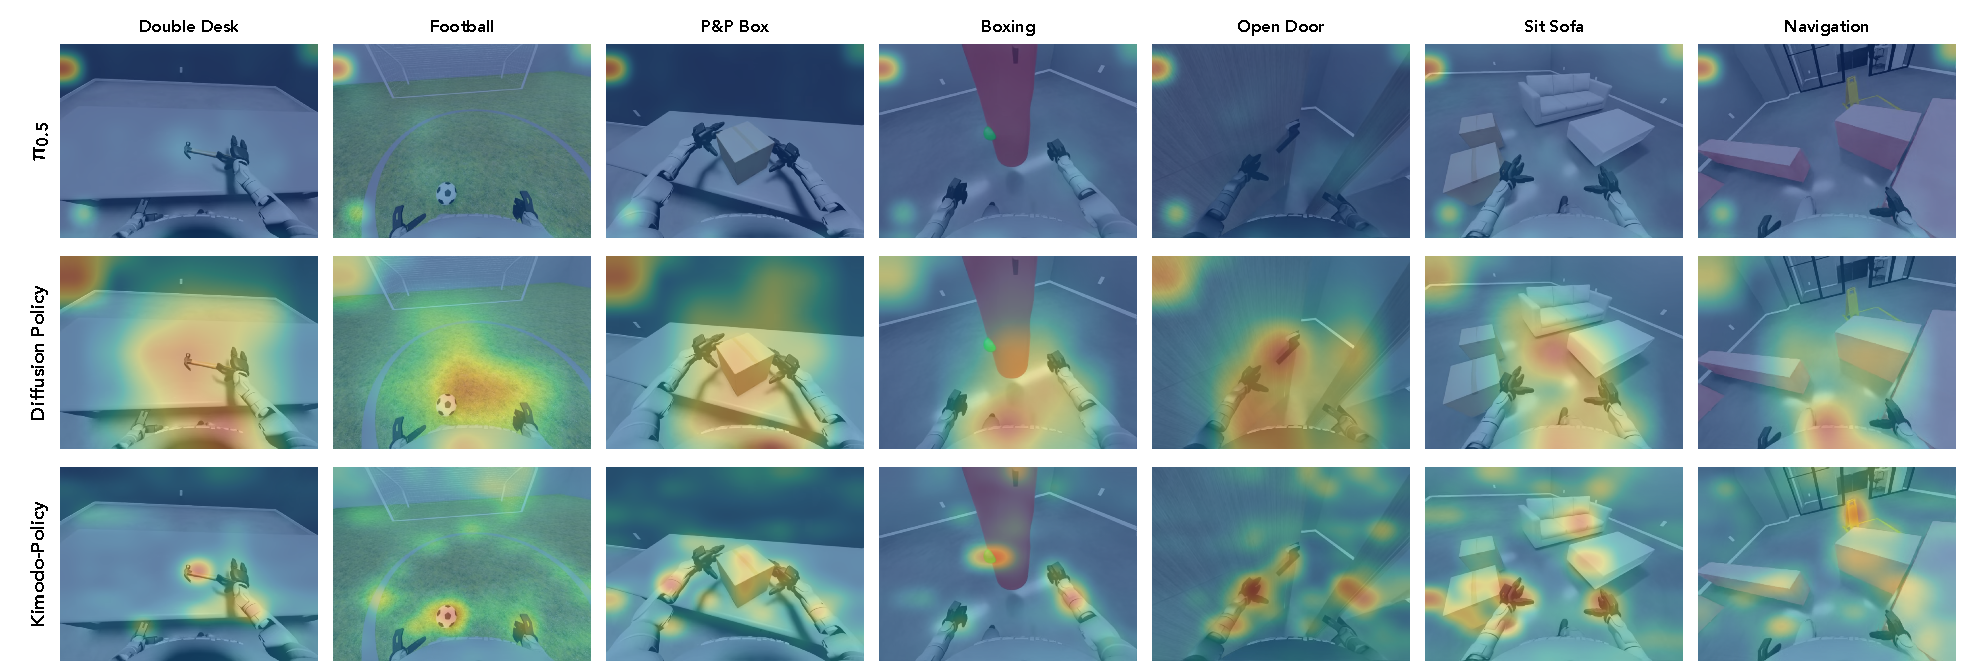
\includegraphics[width=\textwidth]{image/attention.pdf}
  \caption{\textbf{Qualitative Visual Responses Across HumanoidArena Tasks.} Columns show DoubleDesk, Football, P\&Pbox, Boxing, OpenDoor, SitSofa, and VisNavi; rows show $\pi_{0.5}$, Diffusion Policy, and Kimodo-Policy. Kimodo-Policy exhibits localized responses near interaction-relevant regions in the displayed examples.}
  \label{fig:attention}
\end{figure}

\subsection{Evaluation on the SIMPLE Benchmark}
\label{sec:exp_simple}

We next evaluate eight SIMPLE~\citep{simple} tasks covering handover, mobile manipulation, articulated-object interaction, and object pushing (Fig.~\ref{fig:simple_tasks}). An independent Kimodo-Policy$^{*}$ is fine-tuned for each task and evaluated at the L0--L2 randomization levels, which introduce progressively stronger changes in appearance, lighting, and target pose. Table~\ref{table:simple_main_results} reports ten trials per level and task, with RTC disabled for our policies. This evaluation tests whether the motion-based action generator can be adapted to different interaction requirements and remain effective under the prescribed perturbations.

\begin{figure}[H]
  \centering
  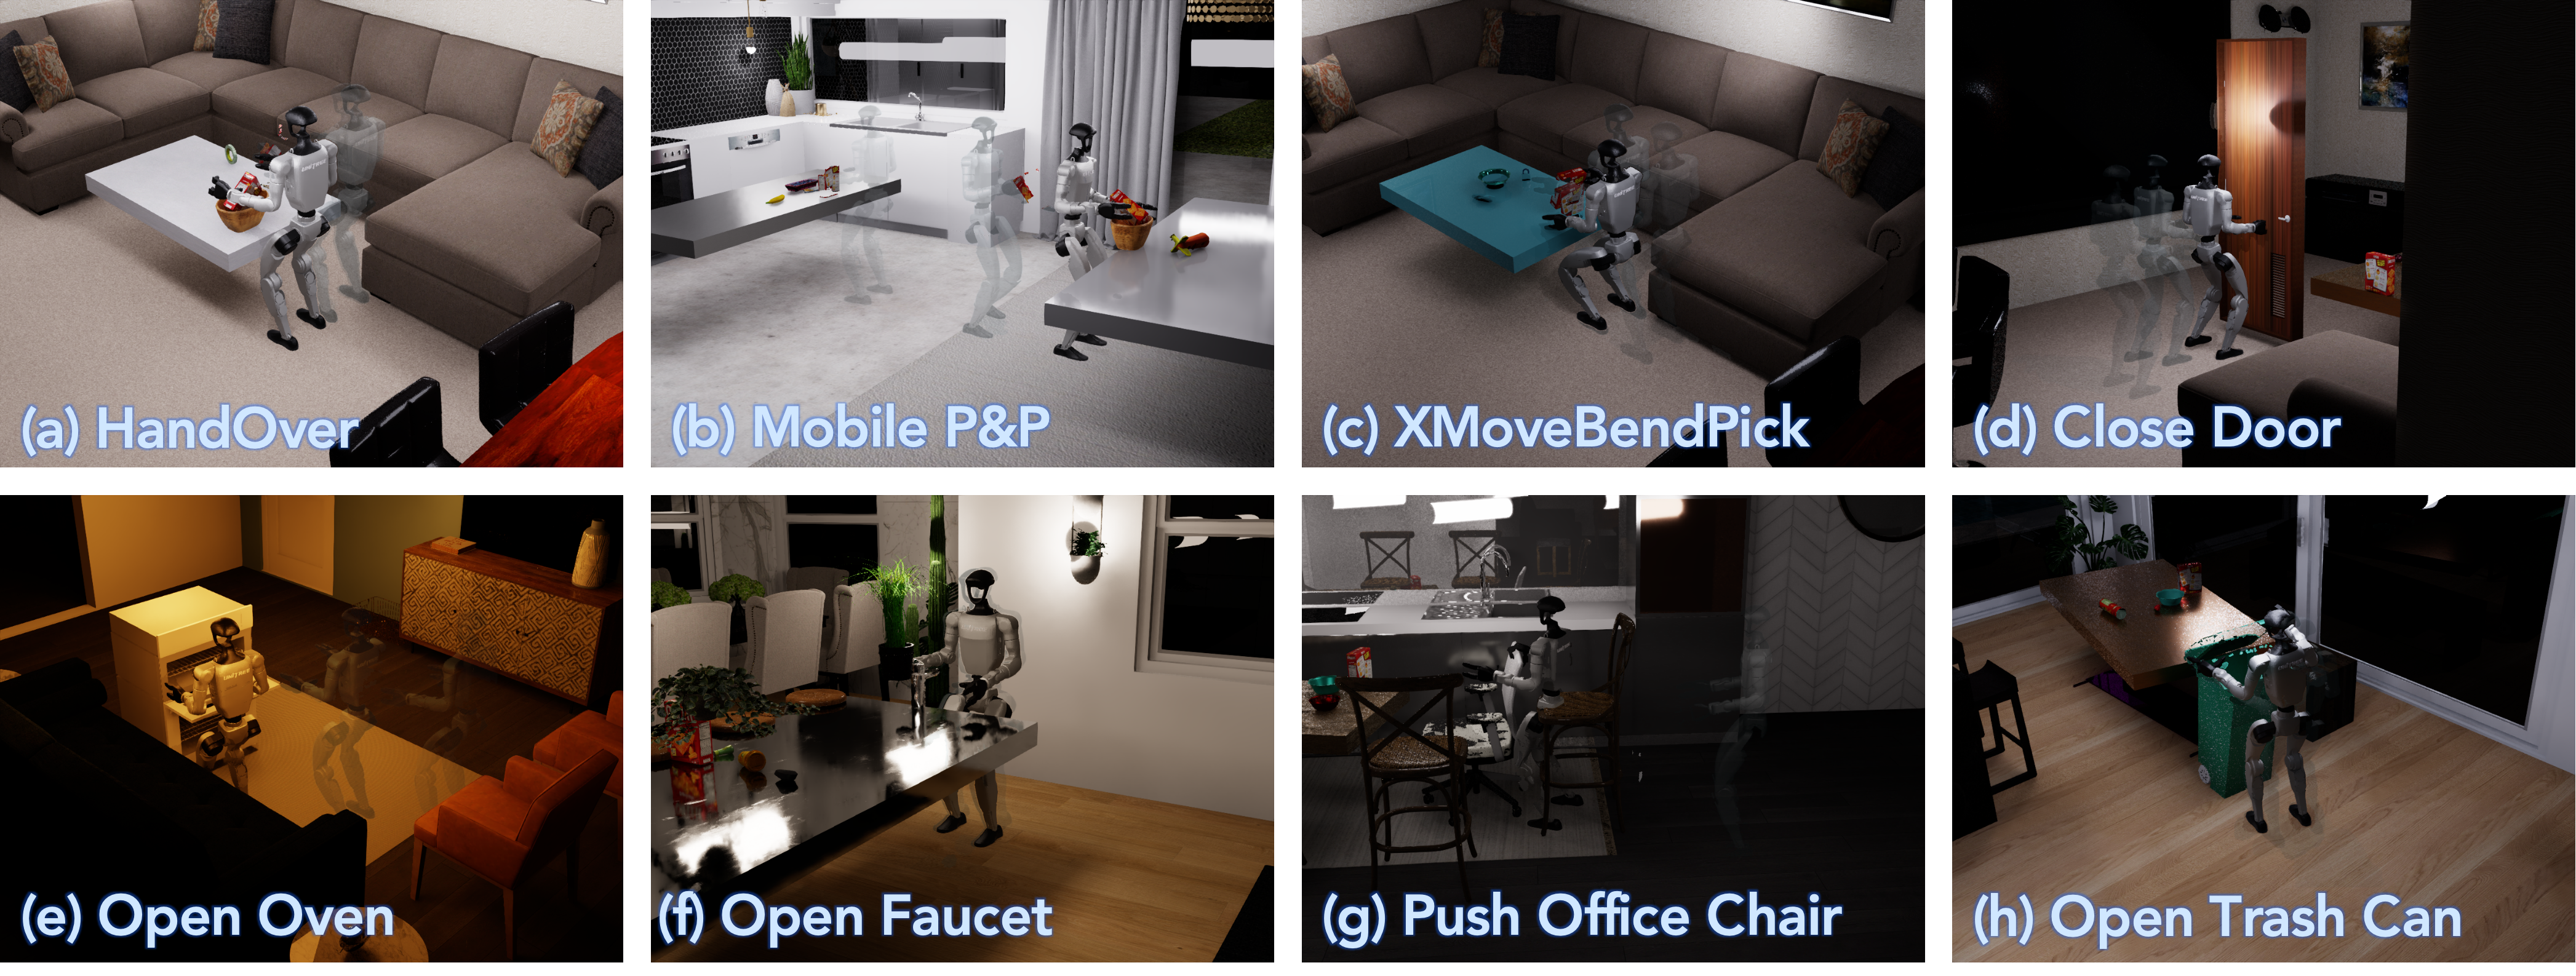
\includegraphics[width=\textwidth]{image/simple.png}
  \caption{\textbf{Evaluated SIMPLE Task Suite.} The selected tasks cover object handover and mobile pick-and-place, locomotion-integrated object pickup, articulated-object interaction, and household-object manipulation. Panels show (a) Handover, (b) Mobile P\&P, (c) XMoveBendPick, (d) CloseDoor, (e) OpenOven, (f) OpenFaucet, (g) Push Office Chair, and (h) OpenTrashCan.}
  \label{fig:simple_tasks}
\end{figure}

\begin{table}[!b]
  \caption{
    \textbf{\textit{Single-Task Results on SIMPLE.}} L0, L1, and L2 denote evaluation settings with progressively stronger visual and lighting variation and target-pose randomization, from the least perturbed setting (L0) to the most perturbed setting (L2). Each entry reports the number of successful trials at L0/L1/L2, followed in parentheses by the aggregate success rate across all three levels. Baseline results in the first three task columns are from the official SIMPLE repository; the last five $\Psi_0$ results are from Table~7 of the initial SIMPLE report~\citep{simple}. For ACT, $\pi_{0.5}$, EgoVLA, InternVLA-M1, and DP, results in the last five task columns are taken from Table~I of \citet{chen2026memorybeforegoal}. Avg is the mean success rate across all eight tasks, computed from the trial counts. Baseline rows compile results from these sources rather than a unified reevaluation; training and execution settings follow the respective reports. Rows with missing task results show a dash. Bold and underlined values mark the best and second-best aggregate success rates, respectively.
   Baselines include ACT~\citep{ACT}, DreamZero~\citep{dreamzero}, $\pi_{0.5}$~\citep{pi05}, EgoVLA~\citep{egovla}, GR00T N1.6~\citep{grootn1}, InternVLA-M1~\citep{internvla_m1}, DP~\citep{chi2023diffusionpolicy}, H-RDT~\citep{hrdt}, $\Psi_0$~\citep{psi0}.
  }
  \label{table:simple_main_results}
  \centering
  \arrayrulecolor{hclblue}
  \setlength{\tabcolsep}{0pt}
  \renewcommand{\arraystretch}{1.08}
  \fontsize{6.2}{7}\selectfont
  \newcommand{\taskheader}[1]{{\fontsize{5.55}{6.2}\selectfont\textbf{\textsc{\hspace{2.2pt}#1\hspace{2.2pt}}}}}
  \newcommand{\resultentry}[2]{{\fontsize{5.2}{6}\selectfont\hspace{2.2pt}#1\;(#2)\hspace{2.2pt}}}
  \newcommand{\bestentry}[2]{{\fontsize{5.2}{6}\selectfont\textbf{\hspace{2.2pt}#1\;(#2)\hspace{2.2pt}}}}
  \newcommand{\secondentry}[2]{{\fontsize{5.2}{6}\selectfont\hspace{2.2pt}\underline{#1\;(#2)}\hspace{2.2pt}}}

  \newcommand{\avgentry}[1]{{\fontsize{5.2}{6}\selectfont\hspace{2.2pt}#1\hspace{2.2pt}}}
  \begin{adjustbox}{width=\textwidth}
  \begin{tabular}{@{}c*{9}{c}@{}}
    \toprule
    {\fontsize{5.55}{6.2}\selectfont\textbf{Method}}
    & \taskheader{Handover}
    & \taskheader{Mobile P\&P}
    & \taskheader{XMoveBendPick}
    & \taskheader{CloseDoor}
    & \taskheader{OpenOven}
    & \taskheader{OpenFaucet}
    & \taskheader{Push Office Chair}
    & \taskheader{OpenTrashCan}
    & \taskheader{Avg ($\uparrow$)} \\
    \midrule

    ACT
    & \resultentry{4/4/6}{47\%}
    & \secondentry{6/5/7}{60\%}
    & \resultentry{6/8/8}{73\%}
    & \bestentry{10/10/10}{100\%} & \resultentry{1/0/1}{7\%} & \resultentry{0/0/1}{3\%} & \secondentry{9/10/10}{97\%} & \resultentry{4/4/7}{50\%}
    & \avgentry{54.58\%} \\

    DreamZero
    & \secondentry{7/8/9}{80\%}
    & \resultentry{5/3/3}{37\%}
    & \resultentry{0/0/1}{3\%}
    & - & - & - & - & -
    & \avgentry{-} \\

    $\pi_{0.5}$
    & \resultentry{5/4/5}{47\%}
    & \resultentry{3/3/3}{30\%}
    & \resultentry{0/0/0}{0\%}
    & \secondentry{10/10/9}{97\%} & \resultentry{4/3/6}{43\%} & \resultentry{4/2/0}{20\%} & \resultentry{10/10/6}{87\%} & \resultentry{7/6/5}{60\%}
    & \avgentry{47.92\%} \\

    EgoVLA
    & \resultentry{0/4/3}{23\%}
    & \resultentry{0/0/0}{0\%}
    & \resultentry{3/5/4}{40\%}
    & \resultentry{10/8/10}{93\%} & \resultentry{5/8/2}{50\%} & \resultentry{0/0/0}{0\%} & \secondentry{10/9/10}{97\%} & \resultentry{3/5/4}{40\%}
    & \avgentry{42.92\%} \\

    GR00T N1.6
    & \resultentry{1/3/3}{23\%}
    & \resultentry{0/0/0}{0\%}
    & \resultentry{4/4/1}{30\%}
    & - & - & - & - & -
    & \avgentry{-} \\

    InternVLA-M1
    & \resultentry{0/0/0}{0\%}
    & \resultentry{0/0/0}{0\%}
    & \resultentry{3/5/7}{50\%}
    & \resultentry{0/0/0}{0\%} & \bestentry{8/6/8}{73\%} & \resultentry{0/0/0}{0\%} & \resultentry{2/3/1}{20\%} & \resultentry{0/0/0}{0\%}
    & \avgentry{17.92\%} \\

    DP
    & \resultentry{3/2/4}{30\%}
    & \resultentry{4/0/0}{13\%}
    & \resultentry{0/0/0}{0\%}
    & \bestentry{10/10/10}{100\%} & \resultentry{0/0/0}{0\%} & \secondentry{2/3/6}{37\%} & \resultentry{10/6/8}{80\%} & \resultentry{4/7/7}{60\%}
    & \avgentry{40.00\%} \\

    H-RDT
    & \resultentry{0/1/0}{3\%}
    & \resultentry{0/0/0}{0\%}
    & \resultentry{0/0/0}{0\%}
    & - & - & - & - & -
    & \avgentry{-} \\

    $\Psi_0$
    & \secondentry{7/7/10}{80\%}
    & \secondentry{7/5/6}{60\%}
    & \bestentry{10/9/9}{93\%}
    & \bestentry{10/10/10}{100\%}
    & \resultentry{7/5/4}{53\%}
    & \resultentry{3/3/4}{33\%}
    & \bestentry{10/10/10}{100\%}
    & \bestentry{7/9/9}{83\%}
    & \avgentry{\underline{75.42\%}} \\

    \rowcolor{hclbrown!15!white}
    \texttt{Ours}$^{*}$
    & \bestentry{9/8/8}{83\%}
    & \bestentry{9/8/4}{70.0\%}
    & \secondentry{10/7/7}{80\%}
    & \bestentry{10/10/10}{100\%}
    & \secondentry{8/4/5}{57\%}
    & \bestentry{5/6/5}{53\%}
    & \bestentry{10/10/10}{100\%}
    & \secondentry{9/4/6}{63\%}
    & \avgentry{\textbf{75.83\%}} \\

    \bottomrule
  \end{tabular}
  \end{adjustbox}
\end{table}


\textbf{Single-task results.} Kimodo-Policy$^{*}$ achieves 75.83\% mean SR across the eight tasks, compared with 75.42\% for $\Psi_0$~\citep{psi0}, the strongest baseline with complete task coverage. These values correspond to 182 and 181 successful trials out of 240, respectively. Baseline results are compiled from the official SIMPLE release and a subsequent evaluation~\citep{simple,chen2026memorybeforegoal}, as specified in the table caption; they are not a unified reevaluation under our training and execution pipeline. The aggregate performance is therefore comparable, with a small numerical advantage for Kimodo-Policy$^{*}$. Kimodo-Policy$^{*}$ attains the best or joint-best SR on five tasks. It leads on Handover (25/30 successes), Mobile P\&P (21/30), and OpenFaucet (16/30), compared with the strongest baseline counts of 24/30, 18/30, and 11/30, respectively. It also achieves 30/30 on both CloseDoor and Push Office Chair, tying the best reported results. It ranks second on the remaining three tasks: XMoveBendPick (24/30 versus 28/30 for $\Psi_0$), OpenOven (17/30 versus 22/30 for InternVLA-M1~\citep{internvla_m1}), and OpenTrashCan (19/30 versus 25/30 for $\Psi_0$). This distribution demonstrates broad applicability of the motion-based policy while identifying interaction types for which other approaches remain stronger. Averaged across the eight tasks, Kimodo-Policy$^{*}$ achieves 87.50\%, 71.25\%, and 68.75\% SR at L0, L1, and L2, respectively. Performance remains perfect on CloseDoor and Push Office Chair, whereas Mobile P\&P declines from 9/10 at L0 to 4/10 at L2. The adapted policy therefore remains sensitive to perceptual and geometric variation despite its inherited motion prior. Together, these results support competitive task performance while identifying robustness as an important remaining challenge.

\subsection{Evaluation on the Real-World Humanoid Robot}
\label{sec:exp_real}

We deploy Kimodo-Policy on a physical humanoid to evaluate the complete perception--generation--tracking pipeline beyond simulation. The eight tasks require different combinations of locomotion, posture adjustment, single- and dual-arm coordination, and object interaction (Fig.~\ref{fig:real_world}). Each policy is evaluated for ten trials per task. Deployment follows Sec.~\ref{sec:setup_posttraining}, including RTC for Kimodo-Policy. Both Kimodo-Policy variants retain the pretrained motion backbone and differ in whether the trainable modules undergo policy pretraining before task-specific fine-tuning.

\begin{figure}[H]
  \centering
  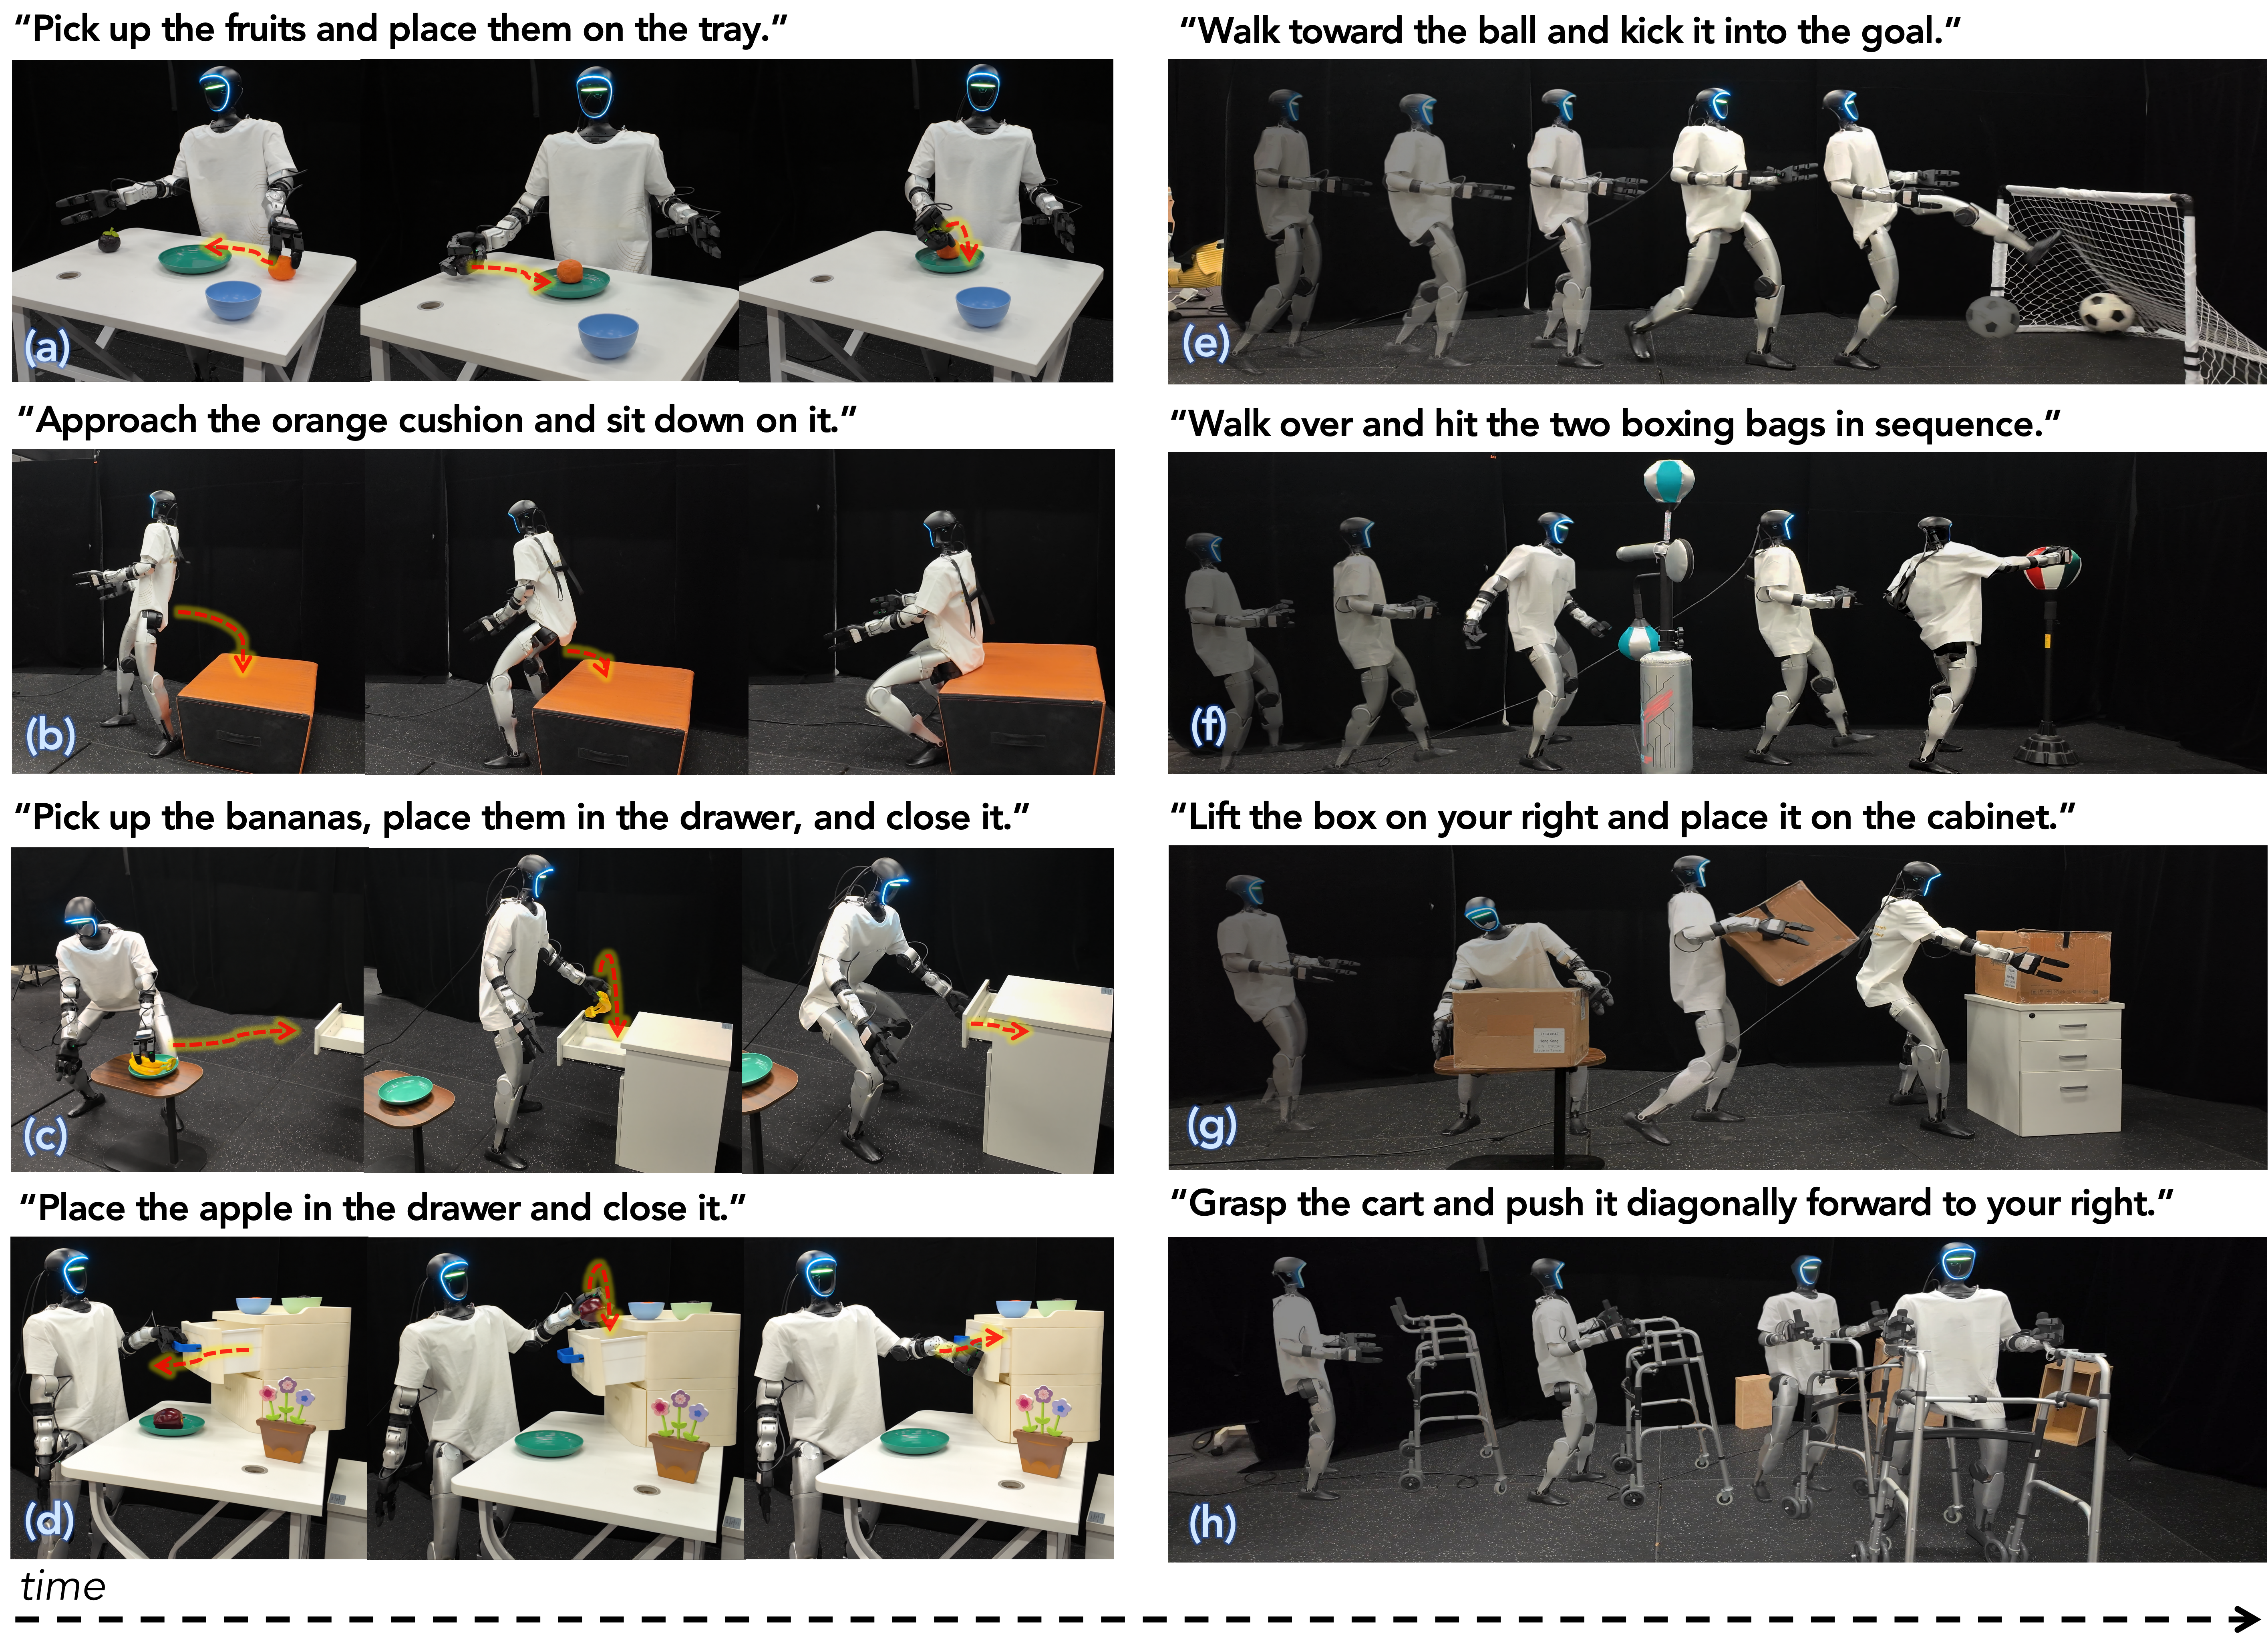
\includegraphics[width=\textwidth]{image/real_world.png}
  \caption{\textbf{Examples of Real-World Humanoid Manipulation.} The image shows representative interaction scenarios involving articulated objects, object transport, and coordinated whole-body motion.}
  \label{fig:real_world}
\end{figure}

\textbf{Real-world results.} As shown in Fig.~\ref{fig:real_world_success_rates}, Kimodo-Policy without additional policy pretraining achieves 45\% mean SR, compared with approximately 31\% for GR00T N1.6~\citep{grootn1} and 35\% for $\Psi_0$. Policy pretraining increases the mean to 60\%, corresponding to 48 successful trials out of 80 and a 15-percentage-point gain over direct fine-tuning. The pretrained variant improves on seven tasks and matches the directly fine-tuned variant on Cart Pushing (60\%). Its highest SRs are 90\% on Punching Bag, 80\% on Cushion Sitting, and 70\% on Dual-Arm PNP. Improvements are largest on Football Scoring (20\% to 50\%), followed by Dual-Arm PNP, Banana Cabinet, and Box Carrying (20 percentage points each). These results provide initial evidence for KAMs on a physical robot. A motion generator conditioned on current observations and coupled to a whole-body tracker supports the evaluated locomotion and manipulation tasks. Because the motion backbone is shared by both variants, their performance difference supports the complementary value of robot-interaction pretraining for adapting the conditioning modules and hand head. The baseline comparison evaluates the deployed systems as a whole; the effect of RTC is not separately ablated. With ten trials per task, the reported rates characterize performance on this evaluation set rather than establish deployment reliability across unrestricted environments.

\begin{figure}[H]
  \centering
  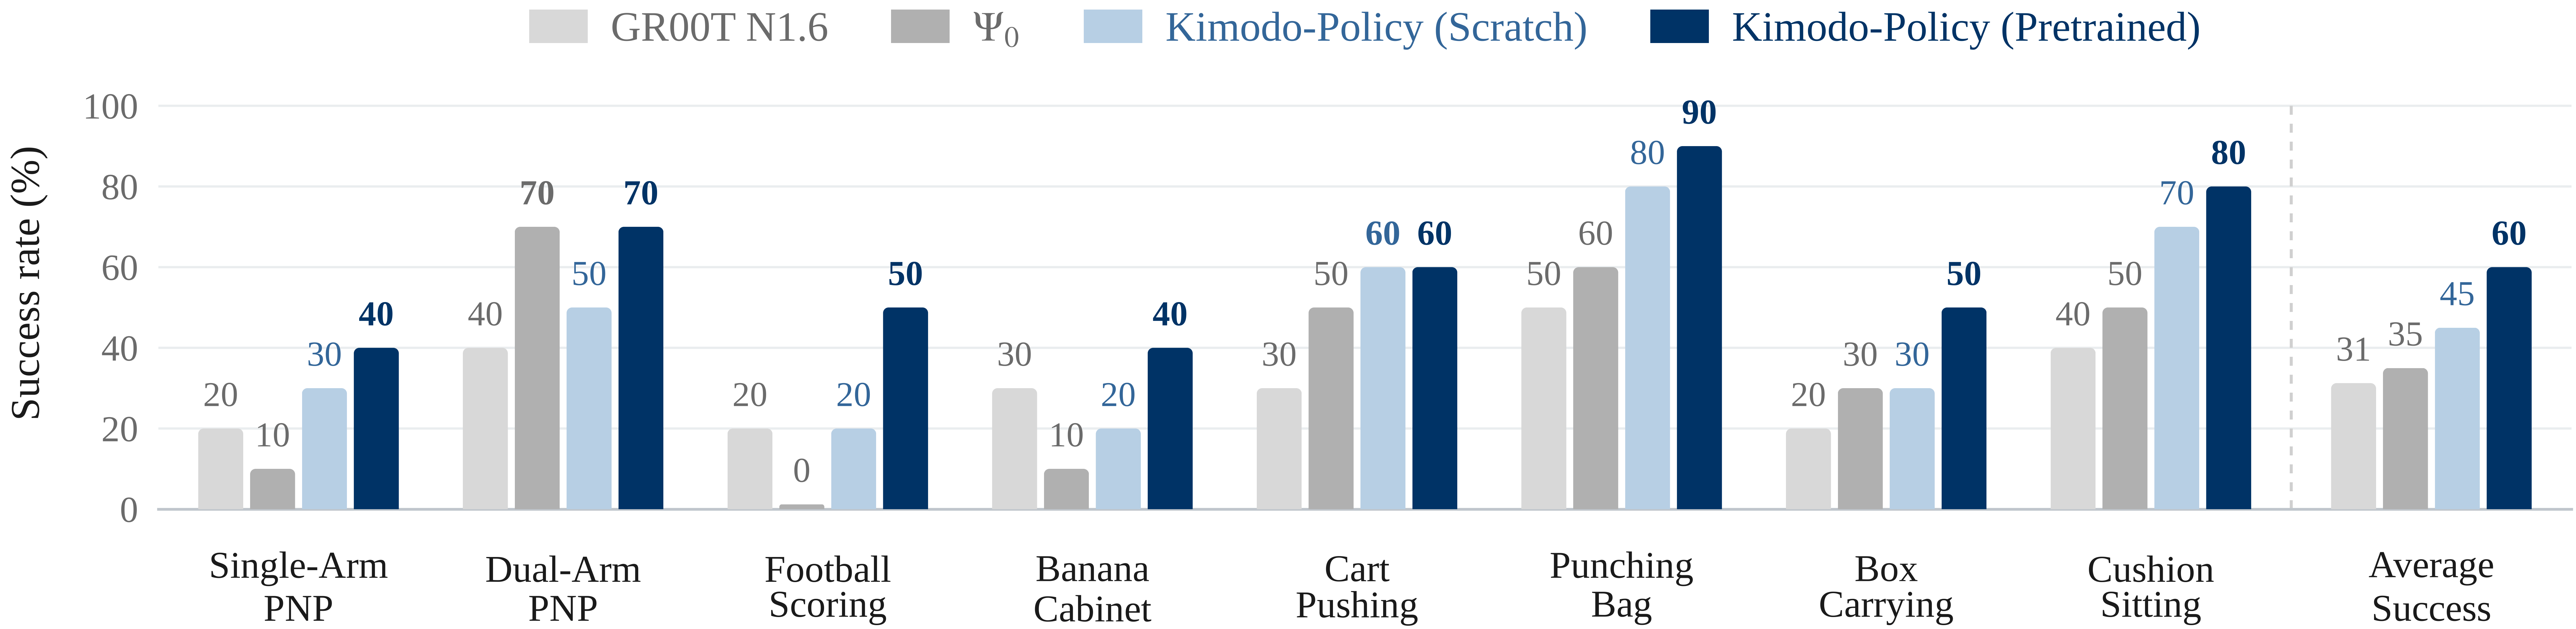
\includegraphics[width=\textwidth]{image/real_world_success_rates.png}
  \caption{\textbf{Real-World Task Success.} Success rates for GR00T N1.6, $\Psi_0$, and Kimodo-Policy with and without additional robot-interaction policy pretraining. Both Kimodo-Policy variants retain the pretrained motion backbone. Each task is evaluated for ten trials; the rightmost group reports the mean across eight tasks. The plot label \emph{Scratch} denotes the variant without additional policy pretraining, while \emph{Pretrained} denotes the variant with it.}
  \label{fig:real_world_success_rates}
\end{figure}

\subsection{How Does the Choice of Motion Prior Affect Downstream Control?}
\label{sec:exp_t2m}

A central implication of KAMs is that the action-generating backbone should matter beyond its parameter count. We examine this by substituting two pretrained Kimodo-G1 variants~\citep{kimodo} while retaining the policy architecture, adaptation procedure, and HumanoidArena evaluation protocol. Both backbones contain 282M parameters. The released SEED-v1 and RP-v1 checkpoints specify motion corpora of 288 h and approximately 560 h, respectively, with 90\%/10\% train/test splits. This comparison evaluates the downstream consequences of selecting different motion priors at matched backbone capacity.

\begin{table}[H]
  \caption{
    \textbf{\textit{Effect of the T2M backbone on Kimodo-Policy.}} We compare two same-size Kimodo-G1 backbones using the same adaptation protocol. Data scales include the training and test splits; results are mean $\pm$ standard deviation over three seeds.}
  \label{tab:t2m_dependency}
  \centering
  \arrayrulecolor{hclblue}
  \begin{adjustbox}{max width=\textwidth}
  \setlength{\tabcolsep}{3.8pt}
  \renewcommand{\arraystretch}{1.08}

  \begin{tabular}{cccccc|ccccc}
  \toprule
  \multirow{2}{*}{\textbf{Base Model}} &
  \multirow{2}{*}{\textbf{Model Size}} &
  \multirow{2}{*}{\textbf{Data Scale}} &
  \multicolumn{3}{c|}{\textbf{Human--Object Interaction}} &
  \multicolumn{4}{c}{\textbf{Human--Scene Interaction}} &
  \multirow{2}{*}{\textbf{Overall~($\uparrow$)}} \\
  \cmidrule(lr){4-6}
  \cmidrule(lr){7-10}

  & & &
  \textbf{\textsc{Football}} &
  \textbf{\textsc{DoubleDesk}} &
  \textbf{\textsc{P\&Pbox}} &
  \textbf{\textsc{OpenDoor}} &
  \textbf{\textsc{SitSofa}} &
  \textbf{\textsc{Boxing}} &
  \textbf{\textsc{VisNavi}} \\
  \midrule

  \texttt{Kimodo-G1-SEED-v1}
  & 282\,M
  & 288\,h
  & \textbf{50.00$\pm$16.33\%}
  & \underline{33.33$\pm$15.46\%}
  & \underline{75.00$\pm$10.80\%}
  & \underline{60.00$\pm$4.08\%}
  & \underline{90.00$\pm$4.08\%}
  & \textbf{71.67$\pm$8.50\%}
  & \textbf{70.00$\pm$18.71\%}
  & \underline{64.29\%} \\

  \rowcolor{hclbrown!8!white}
  \texttt{Kimodo-G1-RP-v1}
  & 282\,M
  & 700\,h
  & \underline{35.0$\pm$7.1\%}
  & \textbf{40.0$\pm$0.0\%}
  & \textbf{80.0$\pm$4.1\%}
  & \textbf{93.3$\pm$6.2\%}
  & \textbf{96.7$\pm$4.7\%}
  & \underline{66.7$\pm$4.7\%}
  & \underline{61.7$\pm$6.2\%}
  & \textbf{67.63\%} \\

  \bottomrule
  \end{tabular}
  \end{adjustbox}
\end{table}


\textbf{Motion-prior transfer results.} Table~\ref{tab:t2m_dependency} reports an overall SR of 64.29\% for SEED-v1 and 67.63\% for RP-v1, a difference of 3.34 percentage points. The gains are task dependent: RP-v1 improves DoubleDesk, P\&Pbox, OpenDoor, and SitSofa, with the largest increase on OpenDoor (60.0\% to 93.3\%). Conversely, Football declines from 50.0\% to 35.0\%, Boxing from 71.67\% to 66.7\%, and VisNavi from 70.0\% to 61.7\%. The overall improvement is thus driven primarily by the net gain on scene-interaction tasks, rather than a uniform improvement across behaviors. The fixed parameter budget makes this result relevant to the KAM premise: the choice of pretrained motion generator affects downstream control even when policy capacity is unchanged. However, the two corpora differ in both size and content, and Table~\ref{tab:t2m_dependency} does not report an independent motion-generation quality metric. The comparison therefore supports the importance of the inherited motion prior, but does not establish a monotonic relationship between T2M quality and control performance or isolate motion-data scale as the cause of the gain.

\subsection{Scaling Robot-Interaction Data and Trainable Policy Capacity}
\label{sec:exp_scaling}

We examine two ways of strengthening the adaptation of a fixed motion backbone: increasing robot-interaction pretraining data and increasing trainable policy capacity. The data sweep holds the policy architecture and downstream seven-task adaptation protocol fixed. The capacity sweep retains the same pretrained motion backbone, downstream data, and optimization protocol while varying the trainable parameter budget. RTC is disabled throughout. These experiments concern policy adaptation around the motion prior, rather than scaling the motion generator itself.

\begin{figure}[H]
  \centering
  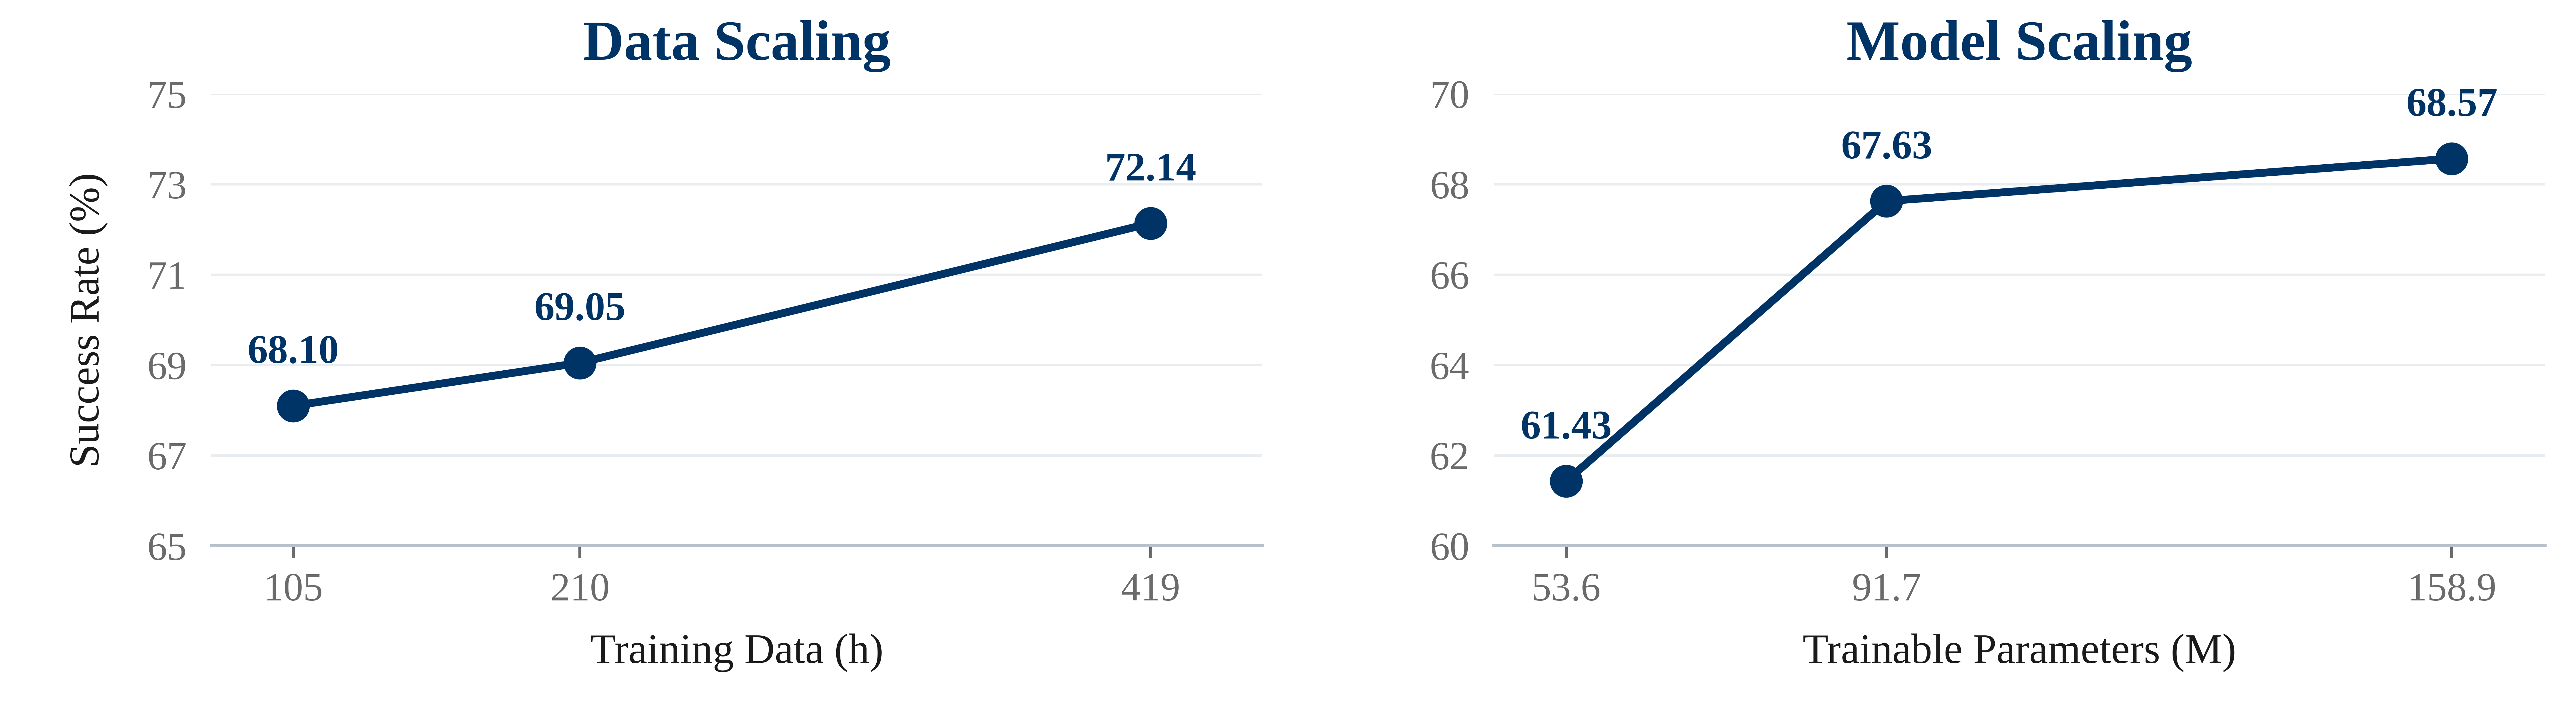
\includegraphics[width=\textwidth]{image/scaling_analysis.png}
  \caption{\textbf{Scaling Policy Adaptation Around a Fixed Motion Backbone.} Overall success on the seven HumanoidArena tasks as a function of robot-interaction policy-pretraining data (left) and trainable policy parameters (right). The motion backbone is held fixed in both sweeps. Each panel follows its respective controlled adaptation setting and should not be interpreted as a joint data--capacity sweep.}
  \label{fig:scaling_analysis}
\end{figure}

\textbf{Scaling results.} Figure~\ref{fig:scaling_analysis} shows that overall SR increases from 68.10\% with 105 h of policy-pretraining data to 69.05\% with 210 h and 72.14\% with 419 h, a total gain of 4.04 percentage points. With the motion backbone fixed, these gains show that additional interaction demonstrations can improve the learned conditioning and hand-control components. This complements the role of motion pretraining in the KAM formulation: an inherited movement repertoire provides a foundation, while robot-interaction data adapt its use to observations and task objectives. The observed increase is consistent across the three evaluated data budgets, although it does not by itself establish a scaling law or predict gains beyond this range. For trainable policy capacity, increasing the trainable parameter count from 53.6M to 91.7M raises overall SR from 61.43\% to 67.63\%; a further increase to 158.9M yields 68.57\%. The total improvement is 7.14 percentage points, with a larger gain in the first increment (6.20 points) than in the second (0.94 points). Thus, downstream performance benefits from additional adaptation capacity within the tested range, with diminishing observed returns. The 91.7M configuration used in the main policy remains within 0.94 points of the largest evaluated configuration while using approximately 42\% fewer trainable parameters. This comparison supports the selected trainable parameter budget; inference efficiency is not measured in this sweep.

\begin{figure}[!b]
  \centering
  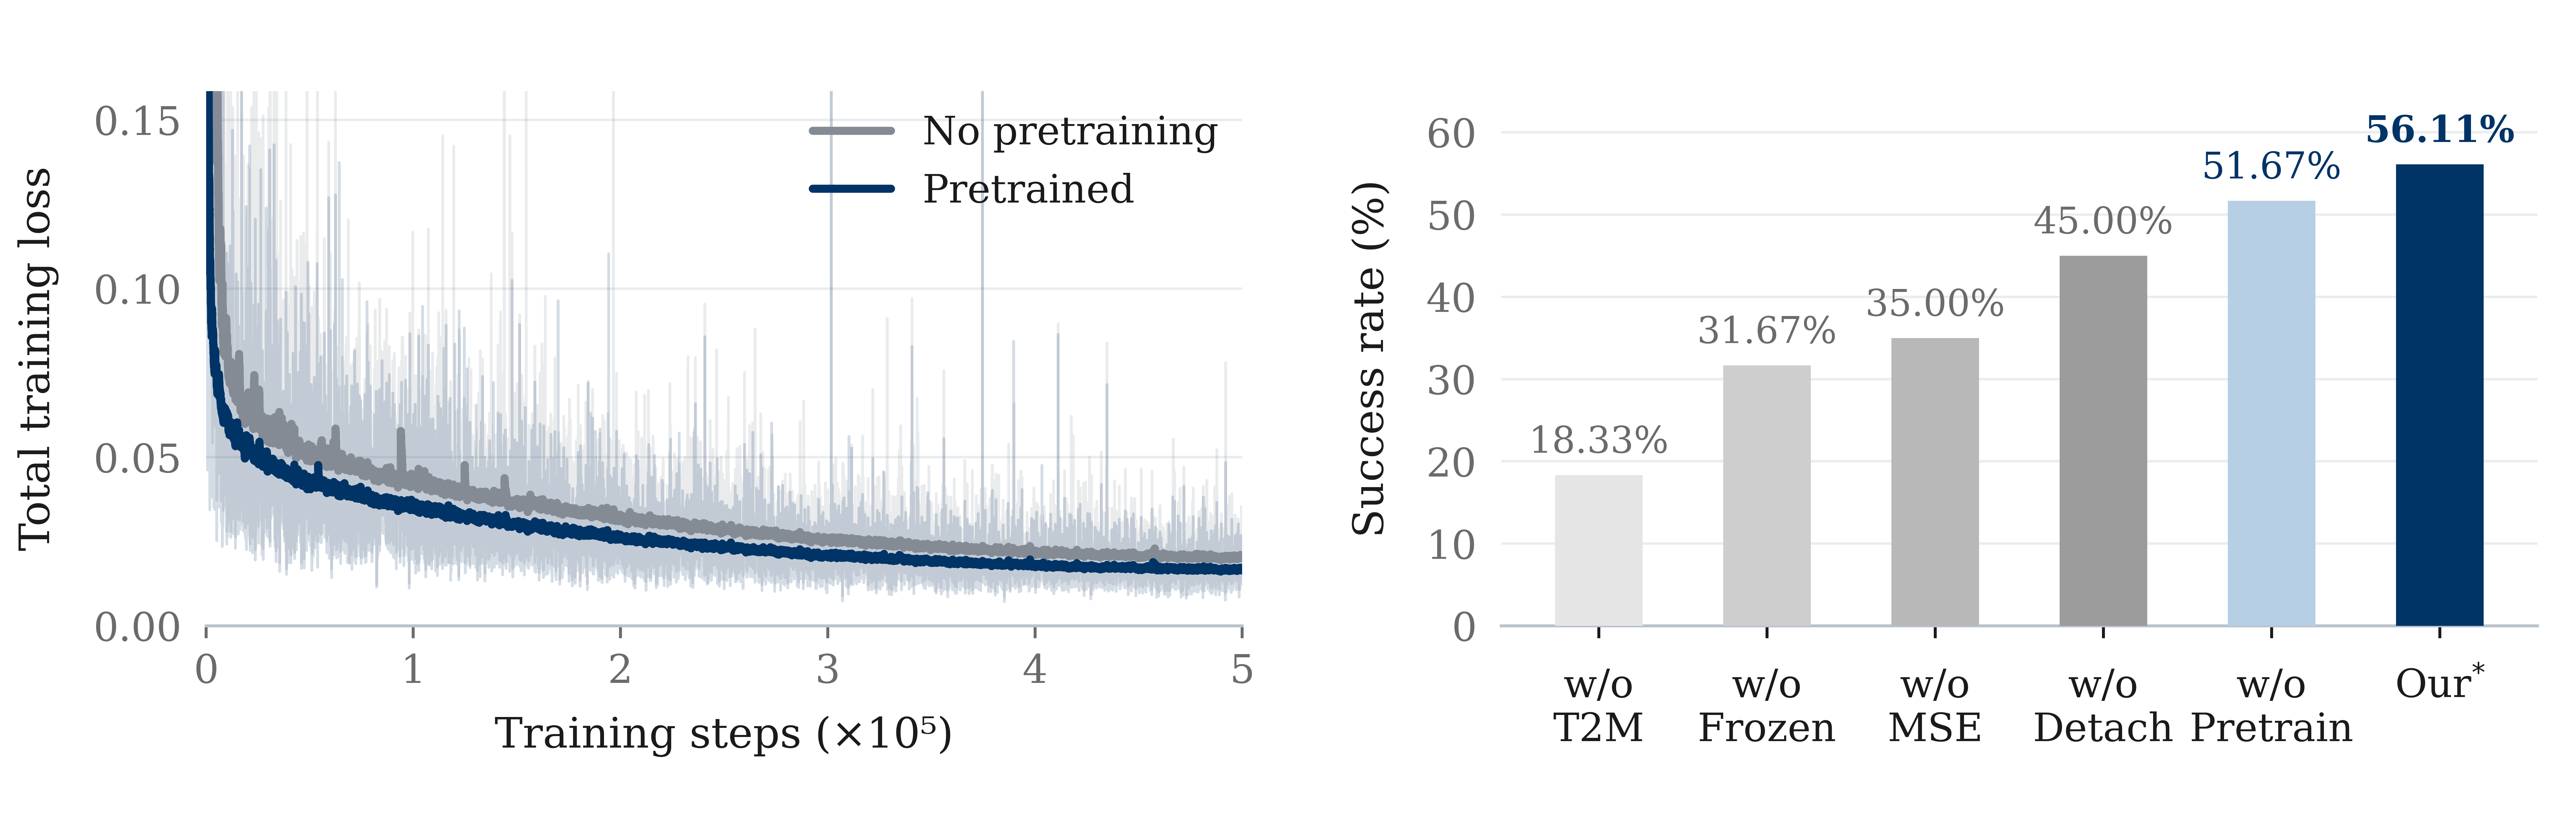
\includegraphics[width=\textwidth]{image/training_loss_comparison.png}
  \caption{\textbf{Policy Adaptation Dynamics and Ablations.} Left: downstream training-loss trajectories with and without additional policy pretraining; both variants retain the pretrained motion backbone. Right: mean success across DoubleDesk, Football, and P\&Pbox after joint seven-task training. Gray bars show independent ablations of the T2M backbone (w/o T2M), backbone freezing (w/o Frozen), the MSE objective (w/o MSE), and root--body gradient detachment (w/o Detach), each relative to the reference without policy pretraining (light blue). Dark blue shows the result with additional policy pretraining.}
  \label{fig:training_loss_comparison}
\end{figure}

\begingroup
\titleformat{\subsection}
  {\normalfont\fontsize{14pt}{17pt}\selectfont\bfseries\color{black}}
  {\thesubsection}{0.55em}{}
\subsection{Ablation Study}
\label{sec:exp_ablation}
\color{black}

We examine the motion backbone, backbone freezing, prediction objective, root--body gradient decoupling, and additional policy pretraining. All variants are trained in the joint seven-task HumanoidArena setting; the ablation metric in Fig.~\ref{fig:training_loss_comparison} averages SR over the three HOI tasks, DoubleDesk, Football, and P\&Pbox. The reference without additional policy pretraining achieves 51.67\%. Each component ablation is compared with this reference, while the effect of policy pretraining is evaluated separately. These three-task averages should be distinguished from the seven-task overall scores in Table~\ref{tab:arena_multi_task}.

\textbf{Ablation results.} The variant labeled w/o T2M achieves 18.33\% SR, 33.34 percentage points below the reference. This is the largest reduction among the evaluated component ablations and supports the importance of the motion-backbone component in this instantiation. Unfreezing the backbone reduces SR to 31.67\%, a 20.00-point drop. Under the evaluated adaptation protocol, retaining the pretrained generator and learning its conditioning through separate trainable branches is therefore more effective than updating the backbone jointly. For the prediction objective, replacing MSE with the original Kimodo motion objective yields 35.00\% SR, 16.67 percentage points below the reference. This favors the direct prediction objective for the evaluated downstream adaptation setting. Separately, removing root--body gradient detachment yields 45.00\%, a reduction of 6.67 points. Detachment preserves the forward dependence of body generation on root predictions while preventing body-stage supervision from updating the root ControlNet. Its benefit shows that forward coordination and coupled optimization need not be implemented through the same gradient pathways. These ablations support the selected objective and gradient boundaries for adapting the hierarchical generator. Finally, additional policy pretraining raises mean SR from 51.67\% to 56.11\%, a gain of 4.44 percentage points. Figure~\ref{fig:training_loss_comparison} also shows generally lower downstream training loss for the pretrained initialization. Since both variants retain the same pretrained motion backbone, the performance gain supports the complementary contribution of learning observation-conditioned interaction before downstream fine-tuning. Taken together, the ablations support a central design principle of this KAM instantiation: preserve a pretrained motion generator, learn how to condition it for interaction, and use task-appropriate objectives and gradient boundaries during adaptation.

\endgroup


\section{Conclusion}
\label{sec:conclusion}

We presented Kimodo-Policy, a humanoid vision–language–action framework that transfers pretrained text-to-motion priors to visually grounded, closed-loop whole-body control. Its root–body–hand architecture combines dedicated motion generators with explicit cross-stage conditioning, accommodating distinct control requirements while maintaining coordinated action generation. Trainable visual branches ground the pretrained motion backbone in the current scene, while motion-history conditioning enables continual replanning from updated observations. Experiments on HumanoidArena, SIMPLE, and eight real-world tasks demonstrate strong performance across diverse locomotion and manipulation scenarios, with only 92M trainable parameters out of 678M total parameters. Further analyses show consistent benefits from stronger T2M backbones, larger VLA pretraining datasets, and increased policy capacity within the evaluated settings. Together, these results establish pretrained motion generators as an effective foundation for humanoid VLA learning, allowing policy adaptation to build on existing coordination and temporal priors when learning task-conditioned interaction.

\textbf{Limitations.} A principal limitation of the current framework is its dependence on a specific low-level motion tracker. Kimodo-Policy is designed and evaluated with SONIC, and its motion-reference interface and deployment pipeline are tailored to this tracker; other tracking controllers are not currently supported. Consequently, the reported results establish the effectiveness of the policy within the SONIC-based control stack, while transfer across trackers remains unverified. Although separating high-level motion generation from low-level execution provides a modular organization, this separation alone does not ensure compatibility with controllers that differ in reference parameterization, tracking behavior, or executable motion range. Extending the framework would therefore require adapting the policy–tracker interface and validating closed-loop performance under the target controller. Developing a more general interface between pretrained motion generation and low-level whole-body control remains an important direction for broadening its applicability.

\textbf{Future Work.} Looking ahead, Kimodo-Policy can be viewed as a motion-prior-informed action expert within a larger multimodal architecture. Integrating it with vision–language models and video generation models, potentially through MoT-style architectures, could combine semantic understanding and visual dynamics modeling with structured whole-body action generation. A complementary direction is to strengthen the underlying motion prior itself. Text–motion supervision can draw on human motion data retargeted to robot embodiments without requiring every sequence to be collected through robot execution with synchronized visual observations, offering a scalable route to motion pretraining. The gains observed with stronger T2M backbones motivate investigating whether broader motion coverage and more capable generators yield further improvements in downstream control. Beyond training robot-space motion models on retargeted data, a longer-term direction is to transfer pretrained human T2M backbones directly into humanoid VLA policies, drawing on the breadth of human motion resources and advances in human motion generation. Such transfer would require aligning motion representations across embodiments and adapting human kinematic priors to robot-specific actuation, balance, and contact constraints. These directions could expand the framework from a standalone policy into a reusable motion-generation component for more capable humanoid systems.

% References cited by the Introduction and experiment tables.

\bibliography{ref}

\end{document}
